\chapter{Proposta}\label{cap:Desenvolvimento}

Para melhor entendimento do processo de pesquisa, organizou-se o fluxograma presente na Figura \ref{fig:fluxogramaPesquisa}.
  
\begin{figure}[H]
\centering
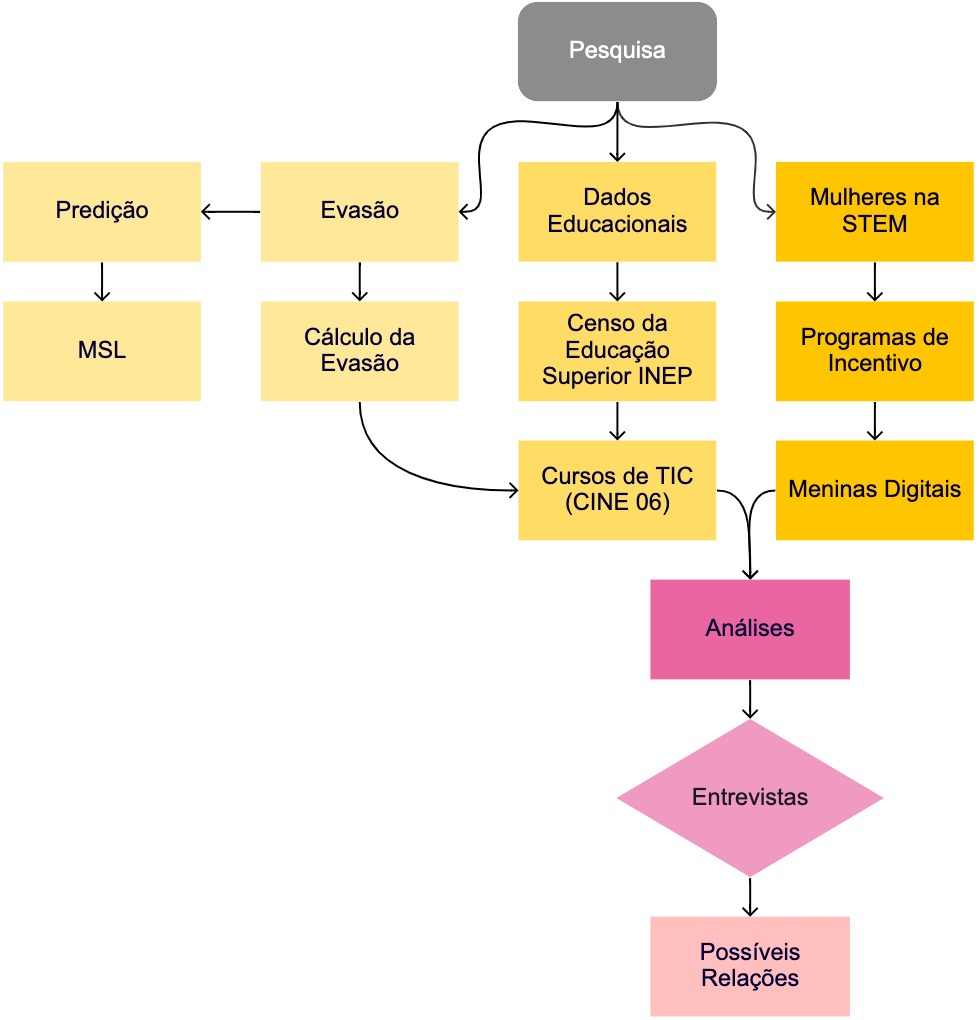
\includegraphics[width=1\textwidth]{Figuras/fluxograma.png}
\caption{Fluxograma do processo de pesquisa}
\label{fig:fluxogramaPesquisa}
\end{figure}

A Figura \ref{fig:fluxogramaPesquisa} apresenta três principais vertentes, a evasão, os dados educacionais e as mulheres na STEM. Inicialmente, a pesquisa foi em busca do estado da arte da predição da evasão, o que resultou no Mapeamento Sistemático da Literatura. 

%%%passar a limpo essa história do mapeamento e quem sabe excluir ele daqui para a defesa final, pois deixa o leitor perdido. Não sei.

Em paralelo, o estudo e exploração dos dados educacionais e do tema mulheres na STEM em busca de um objetivo e fontes de referência. Com isso, tem-se o aprofundamento em cada tema, chegando nos dados do censo da educação superior do INEP, programas de incentivo a presença e permanência de mulheres na área de STEM. Por fim, a partir de análises e entrevistas com os projetos do Programa Meninas Digitais, encontrar uma possível relação entre a presença das mulheres nos cursos de Computação e Tecnologias da Informação e Comunicação e as ações dos projetos parceiros do Programa Meninas Digitais.


\section{Mapeamento Sistemático da Literatura}\label{sec:Mapeamento}


Antes da escolha do tema da presente dissertação o ambiente da evasão foi explorado e além dos trabalhos relacionados encontrados na literatura, um Mapeamento Sistemático da Literatura (MSL) foi produzido em conjunto com o grupo de iniciação científica e está em processo de finalização para submissão. Apresenta-se aqui um panorama geral sobre o MSL.

\subsection{Processo do Mapeamento}\label{sec:procMapeamento}
O MSL realizado segue a diretriz proposta por \citeonline{petersen:2015} que apresenta as seguintes etapas: definição das questões de pesquisa, processo de busca (formulação de string de busca e realização da busca em bases acadêmicas), seleção dos estudos com base em critérios de inclusão e exclusão, análise dos estudos (extração e categorização dos dados) visando responder às questões de pesquisa.

\subsection{Objetivos e Questões de Pesquisa}\label{sec:objQuestoes}
O MSL tem o objetivo de identificar o estado da literatura sobre o estudo da predição de estudantes que possam evadir e a classificação da evasão em diferentes contextos educacionais, este trabalho definiu cinco questões de pesquisa:

\begin{itemize}
\item \textbf{Q1}: Como é definido o conceito de evasão em diferentes contextos educacionais?
\item \textbf{Q2}: Quais são as técnicas e algoritmos utilizados nos estudos sobre a predição da evasão em diferentes contextos educacionais?
\item \textbf{Q3}: Quais são os contextos educacionais em que esses estudos são realizados?
\item \textbf{Q4}: Quais elementos e características são usados como recursos nos modelos de predição?
\item \textbf{Q5}: Quais são os critérios usados para avaliar os modelos e algoritmos de predição?
\end{itemize}

\subsection{Processo de Pesquisa}
As seções a seguir detalham mais sobre como o MSL foi realizado e como os artigos foram selecionados.

\subsubsection{Formulação de string}
O primeiro passo no processo de busca é a formulação da \textit{string} de busca. Três conjuntos de palavras-chave foram escolhidos com base na área de pesquisa:

\begin{itemize}
\item \textbf{Evasão}: palavras relacionadas a evasão.
\item \textbf{Educação}: palavras que fazem referência ao contexto educacional;
\item \textbf{Predição}: palavras-chave relacionadas a predição;
\end{itemize}


Após diferentes testes de palavras chaves, sinônimos e palavras relacionadas, a \textit{string} de pesquisa foi definida como:

\begin{center}
\textit{\textit{(predict*) AND (education* OR academic OR college OR student) AND (dropout OR "drop-out" OR "drop out" OR evasion OR "at-risk" OR "at risk" OR retention OR attrition)}}
\end{center}

Ressalta-se que * é um caractere curinga usado para representar um ou mais caracteres para amplificar os resultados de pesquisa.

A \textit{string} de busca foi aplicada nas bases de dados acadêmicas, também conhecidas como Mecanismos de Buscas Acadêmicas (MBAs), em 22 de novembro de 2021, e a busca foi limitada aos termos presentes nos títulos, resumos ou palavras-chave dos artigos. Os MBAs utilizados foram ACM, El Compendex, IEEE Xplore e Scopus. Essas bases foram escolhidas por serem bases referência na área da computação.

Como resultado, 85 estudos foram obtidos na ACM, 88 estudos no IEEE e 175 estudos no Scopus, totalizando 360 estudos para a fase de seleção.

\subsubsection{Critérios de inclusão e exclusão}

O objetivo deste mapeamento sistemático foi identificar e classificar artigos que pesquisam estudantes de qualquer ambiente de educacional (formal/não formal, virtual/presencial etc) que possam ter perfil de evasão. Os critérios de inclusão foram, portanto:

\begin{itemize}
\item \textbf{CI1}: artigos disponíveis para download;
\item \textbf{CI2}: artigos em inglês ou português, sendo o português a língua nativa dos autores;
\item \textbf{CI3}: artigos primários;
\item \textbf{CI4}: artigos não duplicados;
\item \textbf{CI5}: artigos completos (apresentam metodologia e discutem seus resultados).
%\item \textbf{CI5}: artigos com experimentos ou simulações relacionados à evasão em diferentes contextos educacionais, apresentam metodologia e discutem seus resultados;
\end{itemize}

Os critérios de exclusão foram:
\begin{itemize}
\item \textbf{CE1}: artigos sem experimentação ou simulação, pois são artigos que se interessam principalmente em descrever um determinado algoritmo ou método, que não tem relação com este estudo;
\item \textbf{CE2}: artigo sem explicação dos resultados, considerando que sem os resultados da pesquisa não seria possível entender o grau de eficiência dos algoritmos utilizados.
\end{itemize}

% \subsection{Análises}

% \subsection{Resultados}




\subsection{Seleção dos Artigos}\label{sec:processoPesquisa}
%Nesta seção Todo o processo de pesquisa pode ser observado no Apêndice \ref{ap:ArtigoPredicao}, mas a seguir busca-se responder superficialmente todas as questões de pesquisa que foram analisadas sobre os 143 artigos encontrados nos Mecanismos de Buscas Acadêmicas (MBA) ACM, El Compendex, IEEE Xplore e Scopus.

%Nesta Seção busca-se responder superficialmente todas as questões de pesquisa que foram analisadas sobre os 142 artigos encontrados nos Mecanismos de Buscas Acadêmicas (MBA) ACM, IEEE Xplore e Scopus. A Tabela \ref{tab:mapeamento} mostra o número de artigos selecionados de acordo com os critérios de inclusão e exclusão.
Após aplicar os critérios de inclusão e exclusão foram analisadas sobre os 142 artigos encontrados nos Mecanismos de Buscas Acadêmicas (MBA) ACM, IEEE Xplore e Scopus. A Tabela \ref{tab:mapeamento} mostra o número de artigos selecionados de acordo com cada um desses critérios.
 
\begin{table}[H]
\centering
\caption{Total de artigos por critério de inclusão e exclusão}
\label{tab:mapeamento}
\resizebox{\columnwidth}{!}{%
\begin{tabular}{llllll}
                                                                                              & \textbf{MBA}                                 & \textbf{Scopus}          & \textbf{ACM}             & \textbf{IEEE}            & \textbf{Total}           \\ \hline
\multicolumn{1}{|l|}{}                                                                        & \multicolumn{1}{l|}{Retorno Inicial}                         & \multicolumn{1}{l|}{289} & \multicolumn{1}{l|}{118} & \multicolumn{1}{l|}{102} & \multicolumn{1}{l|}{509} \\ \hline
\multicolumn{1}{|l|}{\cellcolor[HTML]{C0C0C0}}                                                & \multicolumn{1}{l|}{Artigos disponíveis para download}       & \multicolumn{1}{l|}{277} & \multicolumn{1}{l|}{118} & \multicolumn{1}{l|}{99}  & \multicolumn{1}{l|}{494} \\ \cline{2-6} 
\multicolumn{1}{|l|}{\cellcolor[HTML]{C0C0C0}}                                                & \multicolumn{1}{l|}{Artigos em inglês ou português}          & \multicolumn{1}{l|}{269} & \multicolumn{1}{l|}{111} & \multicolumn{1}{l|}{99}  & \multicolumn{1}{l|}{479} \\ \cline{2-6} 
\multicolumn{1}{|l|}{\cellcolor[HTML]{C0C0C0}}                                                & \multicolumn{1}{l|}{Artigos primários}                       & \multicolumn{1}{l|}{265} & \multicolumn{1}{l|}{107} & \multicolumn{1}{l|}{98}  & \multicolumn{1}{l|}{470} \\ \cline{2-6} 
\multicolumn{1}{|l|}{\cellcolor[HTML]{C0C0C0}}                                                & \multicolumn{1}{l|}{Artigos não duplicados}                  & \multicolumn{1}{l|}{263} & \multicolumn{1}{l|}{100} & \multicolumn{1}{l|}{95}  & \multicolumn{1}{l|}{458} \\ \cline{2-6} 
\multicolumn{1}{|l|}{\multirow{-5}{*}{\cellcolor[HTML]{C0C0C0}\textbf{Critério de Inclusão}}} & \multicolumn{1}{l|}{Artigos completos}                       & \multicolumn{1}{l|}{263} & \multicolumn{1}{l|}{99}  & \multicolumn{1}{l|}{94}  & \multicolumn{1}{l|}{456} \\ \hline
\multicolumn{1}{|l|}{\cellcolor[HTML]{C0C0C0}}                                                & \multicolumn{1}{l|}{Artigos sem experimentação ou simulação} & \multicolumn{1}{l|}{70}  & \multicolumn{1}{l|}{62}  & \multicolumn{1}{l|}{57}  & \multicolumn{1}{l|}{160} \\ \cline{2-6} 
\multicolumn{1}{|l|}{\multirow{-2}{*}{\cellcolor[HTML]{C0C0C0}\textbf{Critério de Exclusão}}} & \multicolumn{1}{l|}{Artigos sem explicação dos resultados}   & \multicolumn{1}{l|}{62}  & \multicolumn{1}{l|}{55}  & \multicolumn{1}{l|}{54}  & \multicolumn{1}{l|}{142} \\ \hline
                                                                                              &                                                              &                          &                          & Total                    & 142                     
\end{tabular}%
}
\end{table}

Os 142 artigos selecionados são descritos na Tabela \ref{tab:mapeamentoArtigos} disposta no Apêndice \ref{ap:tabelaApendiceMSL}, onde a primeira coluna indica o número de identificação e a segunda coluna a referência completa e estão ordenados alfabeticamente pelo título do artigo.


Com os 142 artigos definidos e expostos, a subseção \ref{sub:Resultados} apresenta de forma resumida a resposta das questões de pesquisa. O processo de seleção foi realizado por um grupo de pesquisadores que contou com a mestranda deste trabalho e 4 estudantes da iniciação científica, todos apoiados por uma pesquisadora sênior. Cada artigo foi avaliado por 2 pesquisadores, os quais observaram separadamente 26 características dos artigos selecionados para depois compararem os resultados encontrados e fazerem uma discussão caso encontrassem disparidades. 

As características observadas foram: Título do artigo, autores, qual local foi publicado, ano de publicação, em qual MBA foi encontrado, qual critério de inclusão se encaixa, qual critério de exclusão, língua, país da universidade dos autores, objetivo do artigo (dividido em 8 categorias gerais), qual conceito de evasão utiliza como base, as técnicas e algoritmos utilizadas para a predição, as dimensões da base de dados, os fatores ou características observados, ensino formal ou informal, ambiente educacional, dados reais ou simulados, duração do estudo, momento da predição, o que avaliou, quais critérios utilizou, os resultados e um item para as observações.


\subsection{Resultados e Discussões}\label{sub:Resultados}

\subsubsection{Q1 - Como é definido o conceito de evasão em diferentes contextos educacionais?}\label{sub:q1}

Para buscar uma definição de evasão nos artigos analisados, fez-se uma nuvem de palavras sobre todos os conceitos adotados, resultando na Figura \ref{fig:nuvemDePalavras}

\begin{figure}[H]
\centering
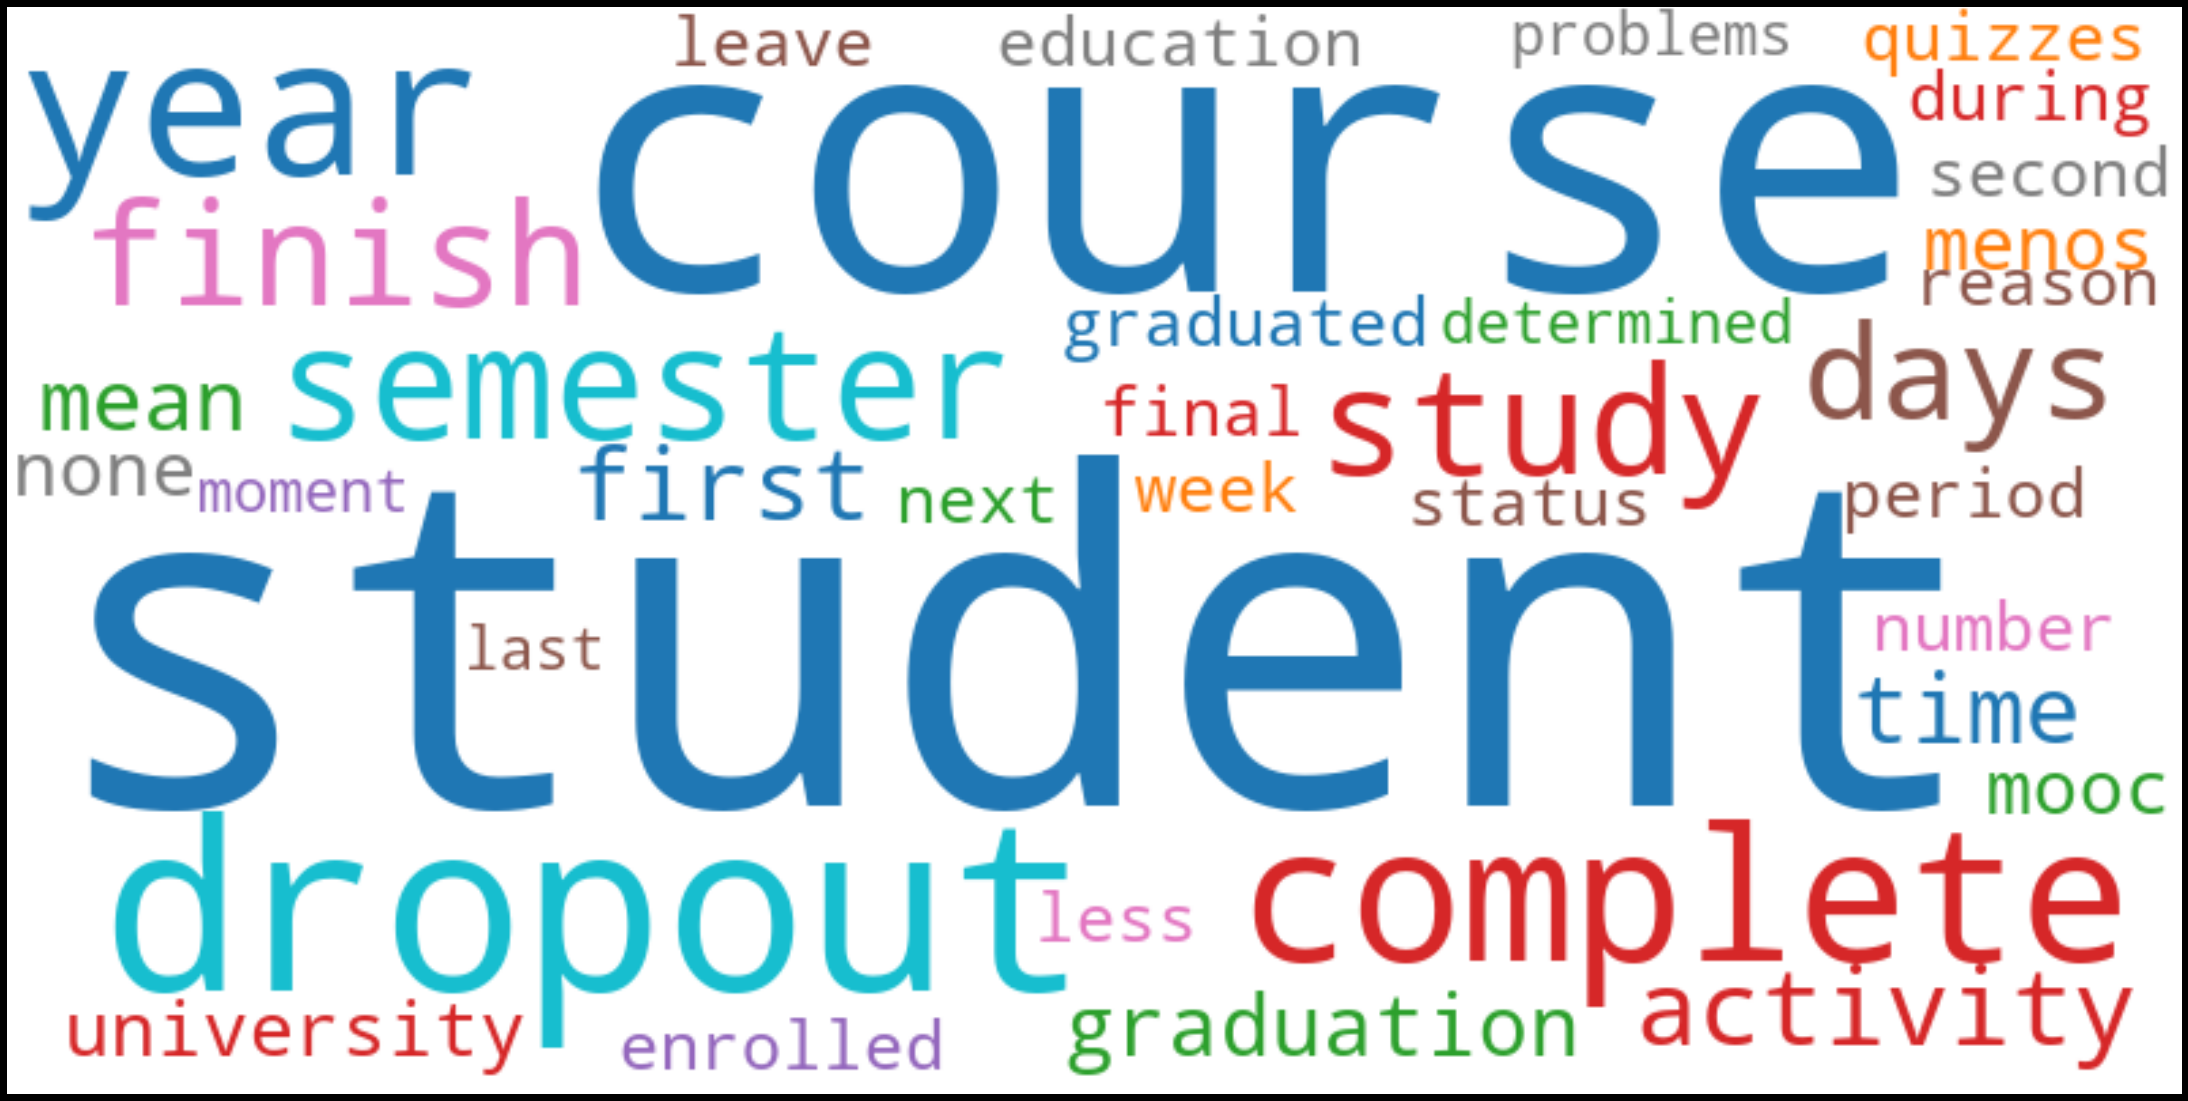
\includegraphics[width=1\textwidth]{Figuras/100_palavras_dropout.png}
\caption{Nuvem de palavras da classificação de evasão}
\label{fig:nuvemDePalavras}
\end{figure}

Observa-se na Figura \ref{fig:nuvemDePalavras} que as palavras mais frequentes nas classificações de evasão são estudante, curso, evasão, semestre, ano, completo, graduado, atividade. Entende-se com isso que no momento de classificar a evasão considera-se ano, semestre, curso com maior frequência que média, problema e quiz, desta forma quando os autores observam a evasão foi mais comum o período/tempo do que rendimento do estudante.

As abordagens mais presentes para a classificação de evasão foram a de abandono do estudo independente do motivo (artigos com ID 22, 23, 48, 70 e 84) e a de estudantes que não completaram o curso em um determinado período de tempo (artigos com ID 1, 6, 25, 37, 49, 57, 78, 83, 85, 88, 100, 115 e 116). No caso de cursos online, estudantes que não interagem com a plataforma por um determinado período de tempo (artigos com ID 4, 19, 26, 31, 42, 75 e 78) também são considerados evadidos.

\subsubsection{Q2 - Quais são as técnicas e algoritmos utilizados nos estudos sobre a predição da evasão em diferentes contextos educacionais?}\label{sub:q2}

Das técnicas, \textit{machine learning} foi de longe a mais utilizada, assumindo 51,4\% sobre todas as outras técnicas citadas. Logo em seguida, as técnicas mistas assumem 21,1\% e técnicas de estatística 10,5\%. As técnicas mistas apresentadas são a utilização de duas ou mais técnicas na mesma abordagem. Quanto aos algoritmos, apresenta-se na Figura \ref{fig:algoritmos} gráfico de barras com os algoritmos mais citados, com destaque para \textit{suport vector machine, decision tree} e \textit{random forest}.


\begin{figure}[H]
\centering
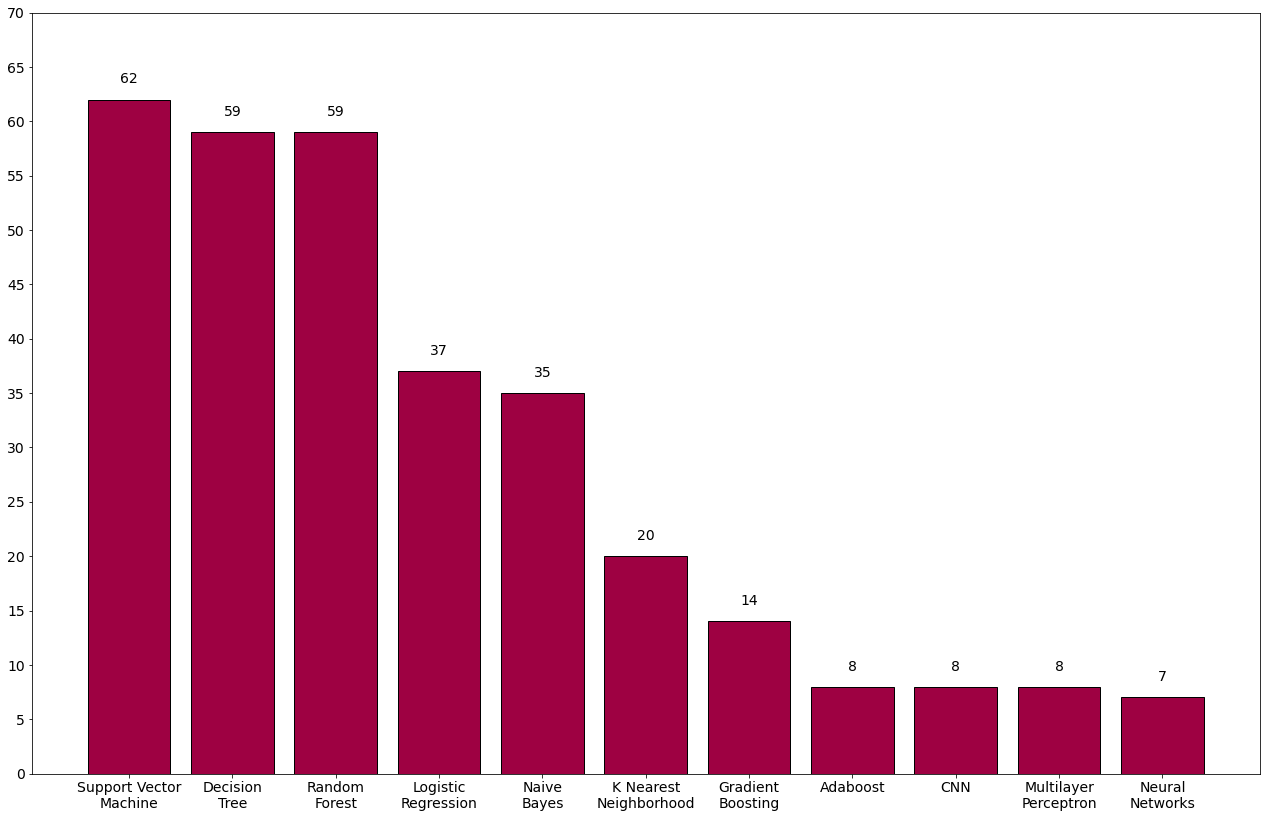
\includegraphics[width=1\textwidth]{Figuras/algoritmos_utilizados.png}
\caption{Algoritmos utilizados para predição da evasão}
\label{fig:algoritmos}
\end{figure}


\subsubsection{Q3 - Quais são os contextos educacionais em que esses estudos são realizados?}\label{sub:q3}

Para responder a questão 3 traz-se a Figura \ref{fig:contexto_ano} que mostra ano a ano o número de artigos por cada contexto educacional abordado. Os conceitos educacionais são classificados como artigos que observaram dados relacionados a certificações, cursos, ensino médio, graduação, mestrado e doutorado.

Na Figura \ref{fig:contexto_ano} dois contextos estão em uma crescente, o contexto de graduação, que também mostra-se predominante e o contexto de cursos.

\begin{figure}[H]
\centering
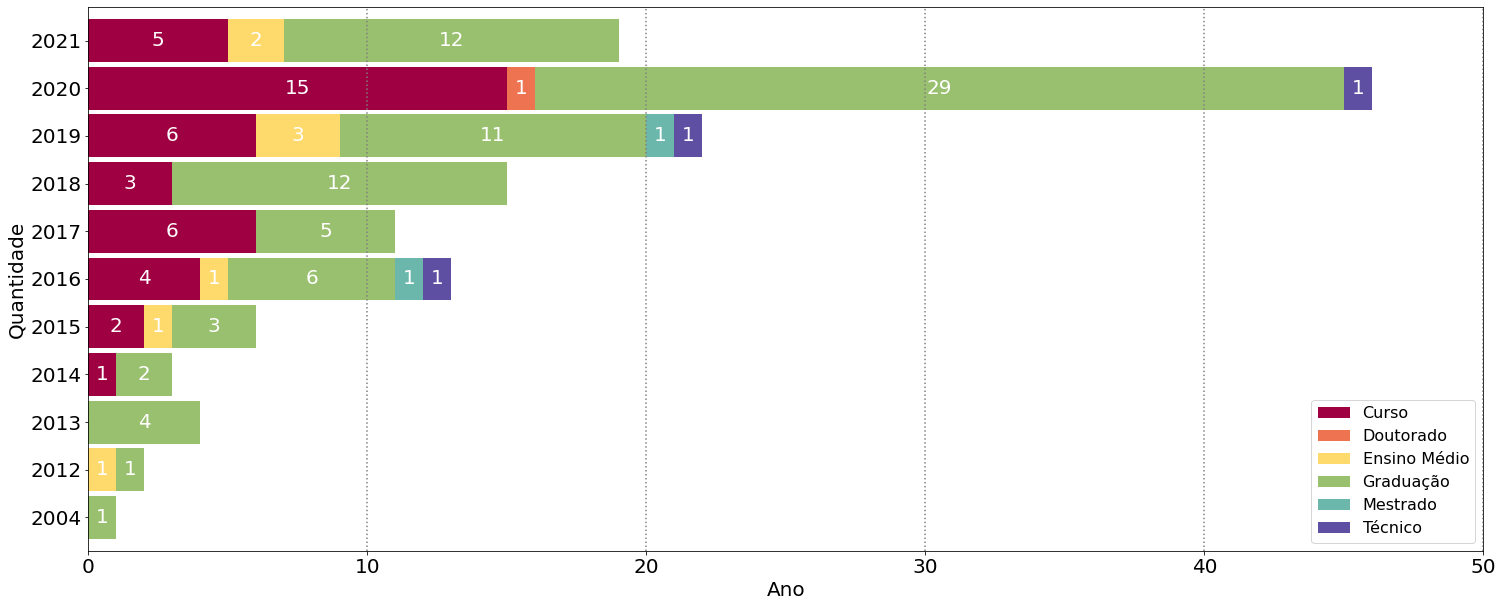
\includegraphics[width=1\textwidth]{Figuras/contexto_ano.png}
\caption{Distribuição de artigos por ano de publicação e contexto}
\label{fig:contexto_ano}
\end{figure}

\subsubsection{Q4 - Quais elementos e características são usados como recursos nos modelos de predição?}\label{sub:q4}

A nuvem de palavra da Figura \ref{fig:nuvemElementosCaracteristicas} mostra quais foram os principais elementos e características utilizadas para aplicar nos modelos de predição.

\begin{figure}[H]
\centering
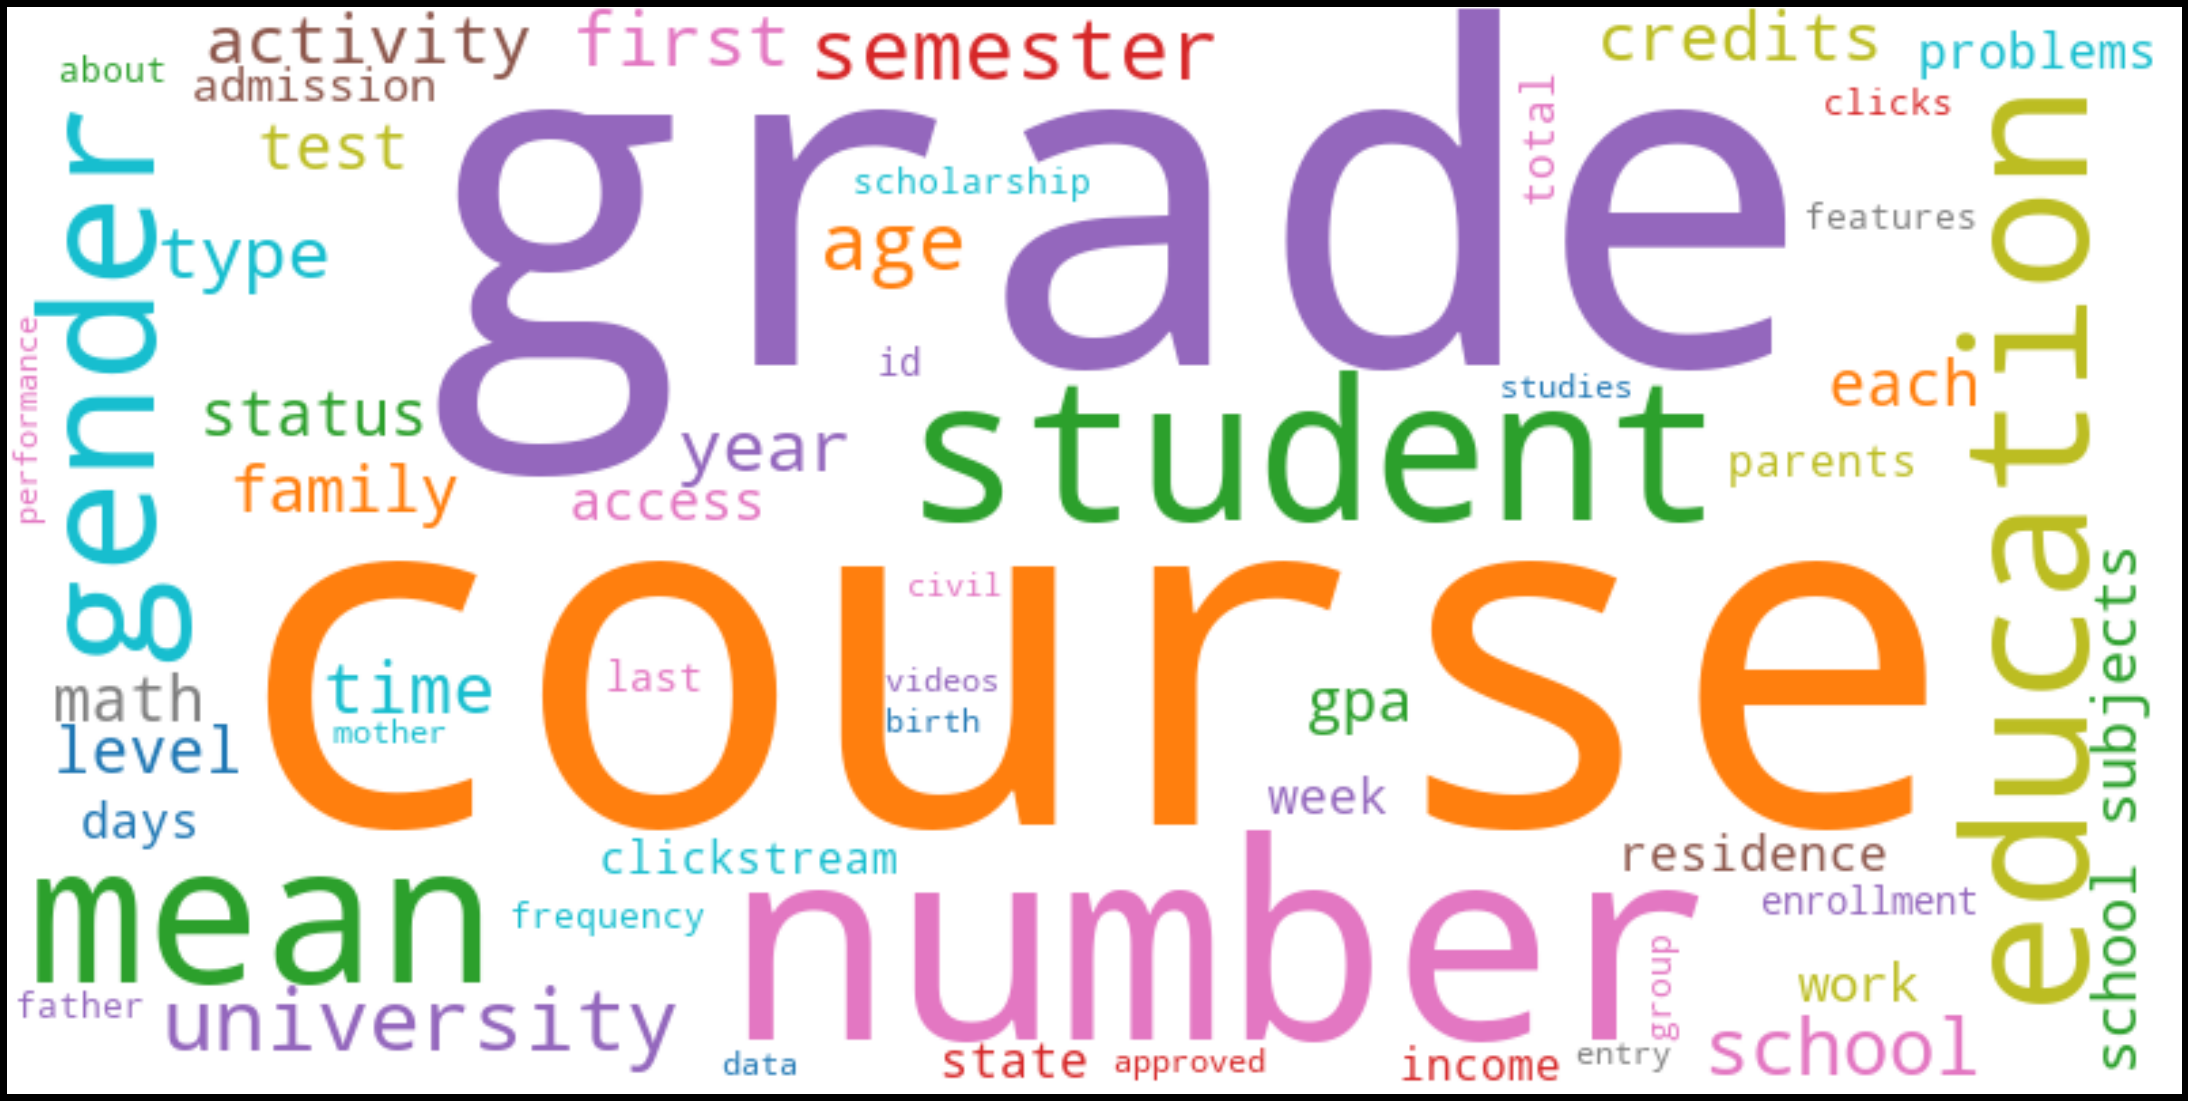
\includegraphics[width=1\textwidth]{Figuras/100_palavras_features.png}
\caption{Nuvem de palavras dos elementos e características usados nos modelos de predição}
\label{fig:nuvemElementosCaracteristicas}
\end{figure}

A nuvem da Figura \ref{fig:nuvemElementosCaracteristicas} mostra que curso é muito considerado e grade também, que do inglês pode significar grade curricular, grau, curso ou até nota, o que faz sentido, pois a maioria dos fatores esta de alguma forma ligada ao curso. 

É interessante observar que média e gênero aparecem basicamente com a mesma frequência, trazendo a importância do gênero na predição da evasão.

Número refere-se a uma série de características, sendo algumas delas: número de semestres cursados antes da evasão, número de créditos, número de disciplinas obrigatórias por semestre, número de novos alunos, número de alunos que evadiram, número de alunos que continuam no curso, número de alunos que se formam, e outros, que foram valores importantes para alguns dos modelos de predição.“Renda”, “bolsa” e “família” referem-se às necessidades, carências financeiras e a aquisição de bolsas mostram influência na evasão dos estudantes. 

Observa-se também fatores relacionados a ensino remoto, “Acesso”, “cliques” e “vídeos”estão associados a quanta interação há entre os estudantes e as mídias digitais ou online disponibilizadas em seus cursos. 

\subsubsection{Q5 - Quais são os critérios usados para avaliar os modelos e algoritmos de predição?}\label{sub:q5}

O critério de avaliação para os modelos e algoritmos que apareceu em maior frequência foi a acurácia, muito possivelmente por conta do que mostrou a Figura \ref{fig:algoritmos}, onde quase todos os modelos são avaliados por meio da acurácia. Logo em seguida vem o critério da precisão como forma de avaliar os modelos de algoritmos de predição. 

Além disso a acurácia é possivelmente a métrica mais simples, onde é calculada com o número de acertos (positivos) divido pelo número total de exemplos.

Observa-se ainda que a maioria dos trabalhos utilizam-se de mais de um critério de avaliação, unindo por exemplo Acurácia, Valor Presente Líquido, Precisão e Revocação na mesma avaliação de algoritmo. 

\subsection{Limitações e Ameaças a validade}\label{sub:limitacoeseameacas}
Para a garantia da qualidade de pesquisa é necessário levantar as limitações e ameaças a sua validade a fim de orientar a reprodutibilidade da pesquisa.

\subsubsection{Viés do Pesquisador}

A pesquisa foi planejada e realizada pelo mesmo grupo de pesquisa, desta forma tudo o que foi produzido pode ter sofrido um direcionamento. Para amenizar este quesito, todos os estudos dos artigos, as análises e respostas as questões de pesquisa foram feitas por pares de pesquisadores. A dupla realizou separadamente seu trabalho e depois fizeram reuniões de consenso. Após os resultados foram discutidos com todo o grupo, inclusive a pesquisadora sênior.

\subsubsection{Viés de amostragem}

A amostra selecionada pode estar nichada a um determinado local não apresentando a população completa, sendo uma ameaça aos resultados do mapeamento. Para a redução deste risco, primeiramente optou-se por mecanismos amplamente utilizados na área de computação e foi feita uma busca com a mesma \textit{string} e no mesmo período

\subsection{Considerações do MSL}
%explicando o tema
Durante a elaboração e análises do MSL, os autores perceberam que um passo atrás era necessário, desta forma nasceram as novas questões relacionadas ao tema desta dissertação, onde não se observa mais os algoritmos de predição da evasão e sim os conceitos e relações a partir do tema evasão. Por isso, a presente Seção apresentou um compilado resumido do que é o mapeamento.

Algumas questões do MSL podem ser tiradas como aprendizado para a atual pesquisa, por exemplo a Questão 1, que busca saber as definições de evasão. Observa-se a importância do gênero para os elementos e características nas variáveis utilizadas nos modelos de predição.
No demais, o MSL mostra-se promissor para sua finalização e possível publicação.


%%%Como resposta desta questão surge a Figura \ref{fig:nuvemDePalavras}, uma nuvem de palavras com estas definições, que podem ser melhor entendidas com a leitura completa do Apêndice \ref{ap:ArtigoPredicao}.

% Para maior completude do estudo, foi realizado um Mapeamento Sistemático da Literatura (MSL). MSLs são definidos como estudos secundários cujo objetivo é fornecer uma visão geral de uma área específica com base em estudos primários e na análise quantitativa das contribuições desses estudos. O principal objetivo de um estudo de mapeamento é fornecer uma visão geral de uma área de pesquisa e classificar a quantidade, forma de pesquisa e possíveis descobertas. Para observar padrões, é comum traçar a frequência de publicação ao longo do tempo \shortcite{petersen:2015}. O presente MSL buscou responder questões mais gerais sobre o tema da evasão.

% \section{Processo de mapeamento}

% O mapeamento sistemático realizado segue a diretriz proposta por \citeA{petersen:2015} que apresenta as seguintes etapas: definição das questões de pesquisa, processo de busca (formulação de strings de busca e realização da busca em bases acadêmicas), seleção dos estudos com base em critérios de inclusão e exclusão, análise dos estudos (extração e categorização dos dados) visando responder às questões de pesquisa. Cada uma dessas etapas é descrita nas próximas subseções.

% \subsection{Questões de Pesquisa}
% Com o objetivo de identificar o estado da literatura sobre o estudo da evasão em diferentes contextos educacionais e a predição de estudantes que possam evadir, este trabalho definiu cinco questões de pesquisa:

% \begin{itemize}
% \item \textbf{Q1}: Como é definido o conceito de evasão em diferentes contextos educacionais?
% \item \textbf{Q2}: Quais são as técnicas e algoritmos utilizados nos estudos sobre a previsão da evasão em diferentes contextos educacionais?
% \item \textbf{Q2}: Quais são os contextos educacionais em que esses estudos são realizados?
% \item \textbf{Q4}: Quais elementos e características são usados como recursos nos modelos de previsão?
% \item \textbf{Q5}: Quais são os critérios usados para avaliar os modelos e algoritmos de previsão?
% \end{itemize}





\section{Entendimento e preparação das bases utilizadas}\label{sec:EntendimentoDados}

Os dados analisados vão até o ano de 2019 pois durante a etapa das análises era o ano mais recende disponível pelo INEP. Além disso, para uma possível atualização, tendo em vista que o censo da educação superior de 2020 foi publicado em março de 2022, seria necessário adaptação e novo entendimento da base, pois novamente o padrão de organização foi alterado, inviabilizando também a forma com que a evasão é calculada na presente dissertação.

Os dados do INEP no momento em que foram baixados estavam disponíveis como apresentados nesta dissertação, porém foram parcialmente retirados do ar no dia 21 de fevereiro de 2022. Para o acesso dos dados mais recentes (referentes ao ano de 2020), o Serviço de Acesso a Dados Protegidos (Sedap) do Governo Federal Brasileiro permite de forma controlada e restrita o acesso às bases, por meio de um conjunto de protocolos, onde os pesquisadores e a sociedade em geral podem ter o acesso às bases de dados relacionadas aos Censos e Avaliações produzidas pela autarquia, exclusivamente para fins de pesquisa e de estudo.

Para analisar a presença das mulheres nos cursos de Computação e Tecnologias da Informação e Comunicação, é necessário observar o contexto dos dados. A presença e permanência das mulheres nesta área pode ser analisada a partir de seu inverso, a evasão e para o início das análises foi preciso dedicar tempo para o entendimento dos dados. Foram três fontes principais de dados, INEP, e-MEC e dados do CINE Brasil. 

Os dados do INEP a partir de 2009 até 2019 totalizam 10 anos de histórico de estudantes, professores e IES. As bases de dados do INEP utilizadas de cada ano são divididas em 6 partes, onde estão guardados os dados gerais do censo, os dados da IES, dos docentes, estudantes, locais e uma tabela auxiliar do CINE. Das 6 partes, as tabelas maiores e mais complexas são as tabelas de estudante e docente, juntas possuem mais de 170 colunas. Como um auxílio o INEP disponibiliza um dicionário de variáveis, para entendimento do que cada coluna significa. No caso dos dados dos estudantes o dicionário de variáveis traz informações das 105 variáveis disponíveis sobre os estudante, algumas delas são:

\begin{itemize}
    \item CO\_CURSO - Código único de identificação do curso gerado pelo E-MEC;
    \item CO\_CINE\_ROTULO - Código de identificação do curso, conforme adaptação da Classificação Internacional Normalizada da Educação Cine/Unesco;
    \item ID\_ALUNO - Código de identificação gerado pelo Inep para o aluno da educação superior;
    \item TP\_COR\_RACA - Tipo da cor/raça do aluno;
    \item TP\_SEXO - Informa o sexo do aluno;
    \item NU\_IDADE - Idade que o aluno completa no ano de referência do Censo;
    \item IN\_DEFICIENCIA - Informa se o aluno é uma pessoa com deficiência, transtorno global do desenvolvimento ou altas habilidades/superdotação;
    \item IN\_INGRESSO\_VESTIBULAR - Informa se o aluno ingressou no curso por vestibular;
    \item IN\_INGRESSO\_ENEM - Informa se o aluno ingressou no curso pelo Enem;
    \item IN\_INGRESSO\_OUTRO\_TIPO\_SELECAO - Informa se o aluno ingressou no curso por outros tipos de seleção;
    \item IN\_ATIVIDADE\_EXTRACURRICULAR - Informa se o aluno participa de algum tipo de atividade extracurricular (estágio não obrigatório, extensão, monitoria e pesquisa).
\end{itemize}

Com a discriminação parcial desta base, é possível observar que ela se correlaciona com as outras duas bases, tanto a do e-MEC na variável CO\_CURSO, quanto a do CINE na variável CO\_CINE\_ROTULO.

As classificações CINE são disponibilizadas pelo INEP em uma tabela auxiliar intitulada TB\_AUX\_CINE\_BRASIL. Para mais detalhes a Diretoria de Estatísticas Edicionais (DEED) disponibiliza o Manual para Classificação dos Cursos de Graduação e Sequenciais que apresenta a estrutura CINE Brasil e todos os procedimentos para classificá-los, tendo como objetivo orientar as IES a realizarem a classificação adequada de seus cursos \cite{CINE}. Com esta classificação, busca-se então os cursos classificados como 06 Computação e Tecnologias da Informação e Comunicação (TIC) pelo CINE.

Já os dados disponíveis pelo e-MEC podem ser pesquisados manualmente onde o usuário tem a opção de fazer uma busca por IES, curso de graduação ou curso de especialização. Escolhendo a busca por curso de graduação é possível buscar a partir do nome do curso, unidade federal, município, gratuidade do curso, modalidade (presencial ou a distância) e grau (bacharelado, licenciatura, tecnólogo ou sequencial).

Como a base do INEP apresenta apenas os códigos de IES e cursos, para levantamento de todos os cursos com seus respectivos nomes é necessário cruzar as informações com a base do e-MEC. Após executar uma busca na base do e-MEC o retorno apresenta-se em formato CSV contendo 56 variáveis, dente elas Código da IES, Sigla da IES, Nome da IES, Código do Curso, Nome do Curso e Código CINE tornando possível conferir e cruzar os dados provindos do INEP e do e-MEC.


O foco nessa dissertação são cursos classificados como 06 Computação e Tecnologias da Informação e Comunicação (TIC) presentes nos dados do INEP dos anos de 2009 a 2019 que estejam relacionados com algum projeto do programa Meninas Digitais.



%--Sabendo disso, o presente trabalho analisa os cursos classificados como 06 Computação e Tecnologias da Informação e Comunicação (TIC).

%A base de dados disponibilizada pelo INEP já sofreu algumas alterações quanto o padrão organizacional, desta forma o presente trabalho utiliza-se dos anos mais próximos desta publicação em que o padrão de dados foi o mesmo, de 2009 a 2019.

%\section{Preparação dos Dados}\label{sec:PreparacaoDados}
%Outro problema de inconsistência de dados foi encontrado no relacionamento entre as bases do INEP e do e-MEC --TABELA COM OS PROJETOS E CÓDIGOS DE CURSOS QUE NAO TEM NA BASE INEP MAS TEM NO EMEC--

Como as bases utilizadas são muito extensas e cheias de informações tornam as analises sobre tais dados ainda mais complexas, cada ano possui em média 2GB. Apesar disso não é necessário o uso completo de todas as informações para cada análise presente na dissertação. Desta forma fez-se uma limpeza inicial, excluindo algumas variáveis para tornar o processo mais rápido e de fácil execução. Outra abordagem utilizada para facilitar o uso das informações é a criação de bases menores, com apenas colunas específicas que estarão em uso para as análises.



\section{Projetos Parceiros do Programa Meninas Digitais}\label{sec:ProjetosLevantados}
Após o levantamento dos dados para as análises da presença, evasão e permanência das mulheres na área de Computação e Tecnologias da Informação e Comunicação, inicia-se a busca pelos projetos do programa Meninas Digitais, que foi o programa escolhido para a presente pesquisa por ser um programa referência no Brasil e na América Latina em equidade de gênero nas carreiras de Tecnologia da Informação e Comunicação.

O programa Meninas Digitais tem como principal objetivo a divulgação da área de computação e suas tecnologias para despertar o interesse de meninas e mulheres. Foi criado no ano de 2011 sob a coordenação da Secretaria Regional da SBC em Mato Grosso e, em 2015, foi institucionalizado pela SBC, recebendo sua chancela, como programa de interesse nacional da comunidade de Computação \cite{meninas:digitais}. O programa surgiu de uma discussão no \textit{Women in Information Technology} (WIT), evento base do Congresso da Sociedade Brasileira de Computação (CSBC) \cite{meninas:digitais}.

Para que a ideia tomasse forma, o Programa conta com a colaboração de multiplicadores de proposta, os Projetos Parceiros (\textit{sister projects}) presentes nas instituições para disseminar a ideia no território nacional.

Todo o processo de mapeamento dos projetos do programa Meninas Digitais ocorreu no dia 2 de abril de 2022 a partir de seu site\footnote{https://meninas.sbc.org.br/projetos/} particular. Organizados na Tabela \ref{tab:ProjetosMeninasDigitais} todas as informações foram retiradas exclusivamente deste site. As informações disponíveis por projetos são nome do projeto, status (projeto ativo ou concluído), ano, contato e endereço, mas nem sempre todas as informações estavam presentes, sua última atualização informada é do dia 13 de junho de 2020.




%%============TABELA===================

\begin{longtable}{|l|l|l|}
\caption{Projetos do Programa Meninas Digitais}
\label{tab:ProjetosMeninasDigitaisD}\\
\hline
\rowcolor[HTML]{C0C0C0} 
\textbf{Nome do Projeto}                                                                                                                                    & \textbf{Status}              & \textbf{Início}                \\ \hline
\endfirsthead
%
\multicolumn{3}{c}%
{{\bfseries Tabela \thetable\ continuação da página anterior}} \\
\hline
\rowcolor[HTML]{C0C0C0} 
\textbf{Nome do Projeto}                                                                                                                                    & \textbf{Status}              & \textbf{Início}                \\ \hline
\endhead
%
  
{\color[HTML]{000000} \#include \textless GURIAS \textgreater{}}                                                                                            & {\color[HTML]{000000} Ativo} & {\color[HTML]{000000} 2018} \\ \hline
  
\#include \textless meninas.uff \textgreater{}                                                                                                              & Ativo                        & 2016                        \\ \hline
  
\#include \textless{}girls\textgreater{}                                                                                                                    & Ativo                        & 2021                        \\ \hline
ADA Code – Meninas Digitais Rondônia                                                                                                                        & Concluído                    & 2017                        \\ \hline
ADAs                                                                                                                                                        & Ativo                        & 2017                        \\ \hline
  
ALICE                                                                                                                                                       & Ativo                        & 2019                        \\ \hline
AmbientAda                                                                                                                                                  & Ativo                        & 2017                        \\ \hline
Android Smart Girls                                                                                                                                         & Concluído                    & 2014-2015                   \\ \hline
  
Aprenda a Programar Jogando                                                                                                                                 & Ativo                        & 2016                        \\ \hline
  
B-Lab Girls                                                                                                                                                 & Ativo                        & 2018                        \\ \hline
Binary Girls                                                                                                                                                & Ativo                        & 2017                        \\ \hline
  
BitGirls                                                                                                                                                    & Ativo                        & 2018                        \\ \hline
  
BitRosa – Elas na Computação                                                                                                                                & Ativo                        & 2015                        \\ \hline
Bits de Ada                                                                                                                                                 & Ativo                        & 2016                        \\ \hline
  
Byte’s Girls                                                                                                                                                & Ativo                        & 2019                        \\ \hline
  
Caliandras Digitais                                                                                                                                         & Ativo                        & 2020                        \\ \hline
  
Catarinas                                                                                                                                                   & Ativo                        & 2016                        \\ \hline
CHICA BYTES                                                                                                                                                 & Ativo                        & 2019                        \\ \hline
  
Cintia (Ciência e Tecnologia da Informação com Elas)                                                                                                        & Ativo                        & 2018                        \\ \hline
Code and Ladies                                                                                                                                             & Ativo                        & 2019                        \\ \hline
Code Queens                                                                                                                                                 & Ativo                        & 2020                        \\ \hline
Code Rosa                                                                                                                                                   & Ativo                        & 2016                        \\ \hline
  
Coletivo Min@                                                                                                                                               & Ativo                        & 2018                        \\ \hline
Compsi Girls                                                                                                                                                & Ativo                        & 2019                        \\ \hline
Computer Girls                                                                                                                                              & Ativo                        & 2016                        \\ \hline
  
Conectadas                                                                                                                                                  & Ativo                        & 2017                        \\ \hline
  
Corte de Lovelace                                                                                                                                           & Ativo                        & 2017                        \\ \hline
CTRL + Gurias                                                                                                                                               & Ativo                        & 2017                        \\ \hline
  
Cunhantã Digital                                                                                                                                            & Ativo                        & 2015                        \\ \hline
Cunharandu Bots                                                                                                                                             & Concluído                    & 2013-2015                   \\ \hline
  
\begin{tabular}[c]{@{}l@{}}DAMA – Disseminação e Apoio à participação de \\ Mulheres na Área de Computação\end{tabular}                                     & Ativo                        & 2020                        \\ \hline
\begin{tabular}[c]{@{}l@{}}Desenvolvimento do Raciocínio Lógico no \\ Ensino Fundamental e Médio\end{tabular}                                               & Ativo                        & 2013                        \\ \hline
  
Developer Girls                                                                                                                                             & Ativo                        & 2017                        \\ \hline
Digital Girls In Rio                                                                                                                                        & Concluído                    & 2016-2018                   \\ \hline
  
Divas                                                                                                                                                       & Ativo                        & 2015                        \\ \hline
  
Ei Mana!                                                                                                                                                    & Ativo                        & 2018                        \\ \hline
  
Elas Digitais IFSC                                                                                                                                          & Ativo                        & 2019                        \\ \hline
  
Elas++ (elas mais mais)                                                                                                                                     & Ativo                        & 2020                        \\ \hline
  
Emíli@s – Armação em Bits                                                                                                                                   & Ativo                        & 2013                        \\ \hline
Encoding Women                                                                                                                                              & Concluído                    & 2016-2017                   \\ \hline
Entre Adas e Marias                                                                                                                                         & Concluído                    & 2017-2017                   \\ \hline
Fatecanas                                                                                                                                                   & Ativo                        & 2019                        \\ \hline
  
FaTech Girls                                                                                                                                                & Ativo                        & 2017                        \\ \hline
FlorADAs                                                                                                                                                    & Ativo                        & 2021                        \\ \hline
  
ForGirls                                                                                                                                                    & Ativo                        & 2019                        \\ \hline
  
Garotas Applicadas                                                                                                                                          & Ativo                        & 2019                        \\ \hline
  
Garotas Tech dos Sertões de Crateús                                                                                                                         & Ativo                        & 2019                        \\ \hline
  
GECET: Garotas nas Engenharias, Ciências Exatas e Tecnologias                                                                                               & Ativo                        & 2020                        \\ \hline
  
GIRLS POWER IN PROGRAMMING                                                                                                                                  & Ativo                        & 2019                        \\ \hline
Girls’n Code                                                                                                                                                & Ativo                        & 2019                        \\ \hline
GRACE – Garotas na Computação e Empreendedorismo                                                                                                            & Ativo                        & 2017                        \\ \hline
  
GRACE – Grupo de Alunas nas Ciências Exatas                                                                                                                 & Ativo                        & 2018                        \\ \hline
Gurias Digitais                                                                                                                                             & Ativo                        & 2018                        \\ \hline
  
Gurias na Computação                                                                                                                                        & Ativo                        & 2016                        \\ \hline
IF(meninas)\{nas exatas\}                                                                                                                                   & Ativo                        & 2017                        \\ \hline
In4Girls                                                                                                                                                    & Ativo                        & 2019                        \\ \hline
Inclusão Feminina em Carreiras Tecnológicas da UFRN                                                                                                         & Ativo                        & 2020                        \\ \hline
InfoGirl (Evento)                                                                                                                                           & Ativo                        & 2014                        \\ \hline
Inova Kids Prudente                                                                                                                                         & Ativo                        & 2018                        \\ \hline
IT Girls – Garotas na Tecnologia da Informação                                                                                                              & Ativo                        & 2016                        \\ \hline
JoinGirls                                                                                                                                                   & Ativo                        & 2018                        \\ \hline
  
JUMI - Juventudes de Mujeres en Ciencia e Ingeniería                                                                                                        & Ativo                        & 2021                        \\ \hline
  
\begin{tabular}[c]{@{}l@{}}Katie: saindo do buraco negro e impulsionando as \\ meninas na computação\end{tabular}                                           & Ativo                        & 2019                        \\ \hline
KeyTech                                                                                                                                                     & Ativo                        & 2018                        \\ \hline
Link com Elas                                                                                                                                               & Ativo                        & 2019                        \\ \hline
  
Maia – Meninas Aprendendo Inteligência Artificial                                                                                                           & Ativo                        & 2018                        \\ \hline
Manas Digitais                                                                                                                                              & Ativo                        & 2018                        \\ \hline
MannaTeam                                                                                                                                                   & Ativo                        & 2016                        \\ \hline
Maria Bonita nas Ciências                                                                                                                                   & Ativo                        & 2019                        \\ \hline
MariaBIT                                                                                                                                                    & Concluído                    & 2015-2017                   \\ \hline
  
Meninas Cientistas                                                                                                                                          & Ativo                        & 2018                        \\ \hline
Meninas da ECITI                                                                                                                                            & Ativo                        & 2018                        \\ \hline
  
Meninas da Geotecnologia                                                                                                                                    & Ativo                        & 2019                        \\ \hline
Meninas Digitais Arretadas                                                                                                                                  & Ativo                        & 2016                        \\ \hline
Meninas Digitais Cáceres Pantanal Digital                                                                                                                   & Ativo                        & 2017                        \\ \hline
  
Meninas Digitais de Rio Pomba                                                                                                                               & Ativo                        & 2019                        \\ \hline
Meninas Digitais do DF                                                                                                                                      & Ativo                        & 2019                        \\ \hline
  
Meninas Digitais do Sudoeste da Bahia                                                                                                                       & Ativo                        & 2019                        \\ \hline
Meninas Digitais do Vale                                                                                                                                    & Ativo                        & 2018                        \\ \hline
  
Meninas Digitais Dourados – Heroínas Digitais                                                                                                               & Ativo                        & 2018                        \\ \hline
\begin{tabular}[c]{@{}l@{}}Meninas Digitais Empreendedoras: Inserção de mulheres \\ na área de Tecnologia da Computação e seus empreendimentos\end{tabular} & Ativo                        & 2019                        \\ \hline
Meninas Digitais IFMT Campo Novo do Parecis                                                                                                                 & Ativo                        & 2017                        \\ \hline
  
Meninas Digitais IFMT Cuiabá                                                                                                                                & Ativo                        & 2015                        \\ \hline
Meninas Digitais IFMT Tangará da Serra                                                                                                                      & Concluído                    & 2015-2017                   \\ \hline
Meninas Digitais IFSULDEMINAS                                                                                                                               & Ativo                        & 2019                        \\ \hline
  
Meninas Digitais na Baixada Fluminense                                                                                                                      & Ativo                        & 2019                        \\ \hline
  
Meninas Digitais na Computação – UNIJU                                                                                                                      & Ativo                        & 2019                        \\ \hline
  
Meninas Digitais na IENH                                                                                                                                    & Ativo                        & 2019                        \\ \hline
  
Meninas Digitais no Cerrado                                                                                                                                 & Ativo                        & 2016                        \\ \hline
Meninas Digitais Piauí                                                                                                                                      & Ativo                        & 2019                        \\ \hline
  
Meninas Digitais Regional Bahia                                                                                                                             & Ativo                        & 2016                        \\ \hline
  
Meninas Digitais Regional Mato Grosso                                                                                                                       & Ativo                        & 2015                        \\ \hline
  
Meninas Digitais Regional Sergipe                                                                                                                           & Ativo                        & 2018                        \\ \hline
  
Meninas Digitais Regional Sul                                                                                                                               & Ativo                        & 2012                        \\ \hline
  
Meninas Digitais Tchê Missões                                                                                                                               & Ativo                        & 2016                        \\ \hline
Meninas Digitais UFBA                                                                                                                                       & Ativo                        & 2016                        \\ \hline
Meninas Digitais UFMT Cuiabá                                                                                                                                & Ativo                        & 2015                        \\ \hline
  
Meninas Digitais UFSC                                                                                                                                       & Ativo                        & 2013                        \\ \hline
  
Meninas Digitais Vale do Itajaí                                                                                                                             & Ativo                        & 2018                        \\ \hline
  
Meninas High Tech                                                                                                                                           & Ativo                        & 2019                        \\ \hline
Meninas Mais Mais                                                                                                                                           & Ativo                        & 2014                        \\ \hline
Meninas na Ciência da Computação                                                                                                                            & Ativo                        & 2014                        \\ \hline
Meninas na Computação                                                                                                                                       & Ativo                        & 2014                        \\ \hline
Meninas na Computação para Escolas Públicas                                                                                                                 & Ativo                        & 2019                        \\ \hline
Meninas na Computação UNIFAP                                                                                                                                & Ativo                        & 2018                        \\ \hline
  
Meninas Paid’éguas                                                                                                                                          & Ativo                        & 2019                        \\ \hline
  
Meninas Programadoras                                                                                                                                       & Ativo                        & 2021                        \\ \hline
Meninas Também Jogam                                                                                                                                        & Ativo                        & 2015                        \\ \hline
Meninas Tecnológicas                                                                                                                                        & Ativo                        & 2018                        \\ \hline
  
Meninas.comp – Computação Também é Coisa de Menina!                                                                                                         & Ativo                        & 2011                        \\ \hline
  
Mermãs Digitais                                                                                                                                             & Ativo                        & 2020                        \\ \hline
  
Metabotix                                                                                                                                                   & Ativo                        & 2013                        \\ \hline
  
MinasCoders                                                                                                                                                 & Ativo                        & 2015                        \\ \hline
  
Minerv@s Digitais                                                                                                                                           & Ativo                        & 2018                        \\ \hline
Mocinhas da Computação                                                                                                                                      & Ativo                        & 2017                        \\ \hline
Mulheres Exatas                                                                                                                                             & Concluído                    & 2018                        \\ \hline
  
Mulheres na Computação Itapetininga                                                                                                                         & Ativo                        & 2014                        \\ \hline
  
Mulheres na Computação UFERSA                                                                                                                               & Ativo                        & 2019                        \\ \hline
Mulheres na TI: Uma Revisão Sistemática Brasileira                                                                                                          & Ativo                        & 2019                        \\ \hline
Núcleo DevGirl                                                                                                                                              & Ativo                        & 2016                        \\ \hline
  
Paragobyte Girls                                                                                                                                            & Ativo                        & 2017                        \\ \hline
Poesia Compilada                                                                                                                                            & Ativo                        & 2016                        \\ \hline
PrendAdas                                                                                                                                                   & Concluído                    & 2017-2019                   \\ \hline
Programa, Essa Menina!                                                                                                                                      & Ativo                        & 2017                        \\ \hline
ProgramADAs                                                                                                                                                 & Ativo                        & 2018                        \\ \hline
PrograMeninas                                                                                                                                               & Ativo                        & 2020                        \\ \hline
  
PS4W – Programa Sabará for Women                                                                                                                            & Ativo                        & 2019                        \\ \hline
Robô Marias                                                                                                                                                 & Concluído                    & 2016-2017                   \\ \hline
Rock and Code\{Girls\}                                                                                                                                      & Ativo                        & 2018                        \\ \hline
\begin{tabular}[c]{@{}l@{}}Sim, elas podem! Ações para o incentivo do interesse \\ de mulheres pela área da computação.\end{tabular}                        & Ativo                        & 2020                        \\ \hline
  
SIsters – Sororidade em Sistemas de Informação                                                                                                              & Ativo                        & 2020                        \\ \hline
Star Girls                                                                                                                                                  & Ativo                        & 2018                        \\ \hline
SuPyGirls                                                                                                                                                   & Ativo                        & 2016                        \\ \hline
Tech’n Roses                                                                                                                                                & Ativo                        & 2018                        \\ \hline
  
Techmanas                                                                                                                                                   & Ativo                        & 2019                        \\ \hline
Techno Girls                                                                                                                                                & Ativo                        & 2017                        \\ \hline
  
Techno Girls                                                                                                                                                & Ativo                        & 2018                        \\ \hline
  
TIChers                                                                                                                                                     & Ativo                        & 2019                        \\ \hline
Turmalinas Tech                                                                                                                                             & Ativo                        & 2018                        \\ \hline
  
WoMakersCode                                                                                                                                                & Ativo                        & 2015                        \\ \hline
\end{longtable}

%%============TABELA FIM===============



Para a informação ser cruzada com os dados provindos do INEP, o seguinte passo a passo foi seguido:
\begin{enumerate}
\item Consideram-se inicialmente todos os projetos descritos na Tabela \ref{tab:ProjetosMeninasDigitaisD};
\item Desconsiderar os projetos com início a partir de 2019 e superiores por não termos os dados do INEP depois desta data; 
\item Buscar no e-Mec por nome da IES que o projeto se relaciona;
\item Com o retorno dos cursos da respectiva IES, selecionar os cursos da cidade do projeto e que possuem código 06 do CINE;
\item Organizar a tabela de projetos com as novas colunas de código de IES e código de curso;
\item Relacionar as informações com a base do INEP. 
\end{enumerate}



%Para que a informação fosse cruzada com os dados provindos do e-Mec, fez-se uma busca projeto a projeto de acordo com a IES  que o projeto se relaciona para o levantamento dos códigos de cursos classificados como cursos de TIC segundo o CINE e código de IES.

%Com todos os projetos mapeados e seus referentes códigos presentes na base do INEP foi possível fazer análises gerais. Para todas as análises, consideram-se os cursos descriminados na Tabela \ref{tab:ProjetosMeninasDigitaisD} porém desconsideram-se os projetos posteriores a 2019, pois não poderiam ser cruzados com os dados do INEP que até o momento da presente análise vão até 2019.


A primeira análise, observada na Figura \ref{fig:impactoProjetoTotal}, mostra o número de estudantes possivelmente impactados por cada projeto levantado do site. O possível impacto é a soma de todos os estudantes dos cursos de TIC que estiveram na IES que o projeto informa como endereço a partir do ano de início do projeto. Caso no endereço apresentado no site não conste uma cidade específica, foi considerado para este trabalho todos os cursos 06 da IES e não todos os cursos 06 de um campus específico da IES. 

Para melhor entendimento do gráfico da Figura \ref{fig:impactoProjetoTotal} traz-se como exemplo o projeto Cunhatã Digital que é um projeto ativo com início no ano de 2015, como endereço possui a Universidade Federal do Amazonas, Instituto de Ensino Superior FUCAPI e Universidade do Estado do Amazonas e destas IES, 11 cursos classificados como cursos de TIC. Desta forma, para encontrar o valor de possível impacto, soma-se o número de estudantes dos respectivos 11 cursos dos anos de 2015 a 2019, totalizando assim 13505 estudantes.

A Figura \ref{fig:impactoProjetoTotal}, apresenta os 30 projetos com maior número de estudantes em TIC e está ordenado por projetos que possivelmente mais impactam mulheres. 

\begin{figure}[H]
\centering
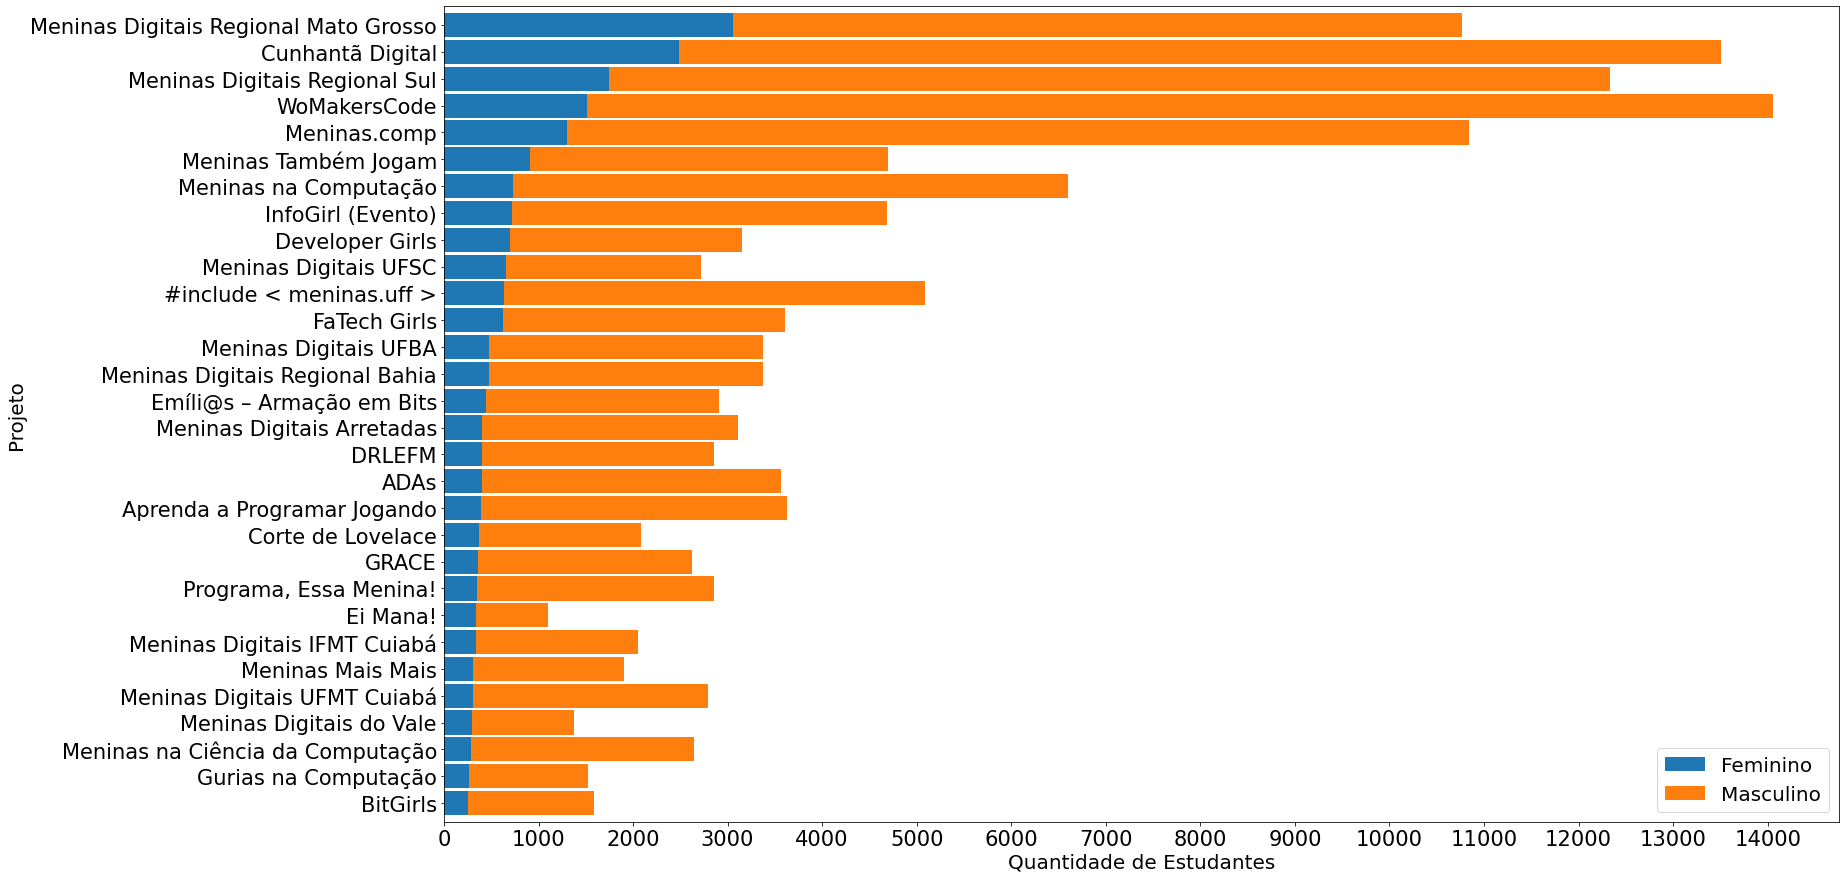
\includegraphics[width=1\textwidth]{Figuras/impacto_projetotrinta.png}
\caption{Número de estudantes possivelmente impactados por sexo e projeto}
\label{fig:impactoProjetoTotal}
\end{figure}

Como a descrição do que considera-se possível impacto, é nítido que o endereço, ano de início do projeto e quantidade de cursos classificados como TIC influenciam esta variável.

O gráfico da Figura \ref{fig:impactoAnoTotal} soma os possíveis impactos ano a ano. Observa-se uma crescente significativa a partir de 2014, e é possível relacionar com o número de projetos do Programa Meninas Digitais. Até o ano de 2014 existiam 13 projetos do Programa Meninas Digitais. Em 2015 mais 11 projetos foram iniciados, em 2016, 20 projetos foram iniciados, em 2017, 19 projetos, em 2018, 29 projetos e em 2019, 34 projetos. 


\begin{figure}[H]
\centering
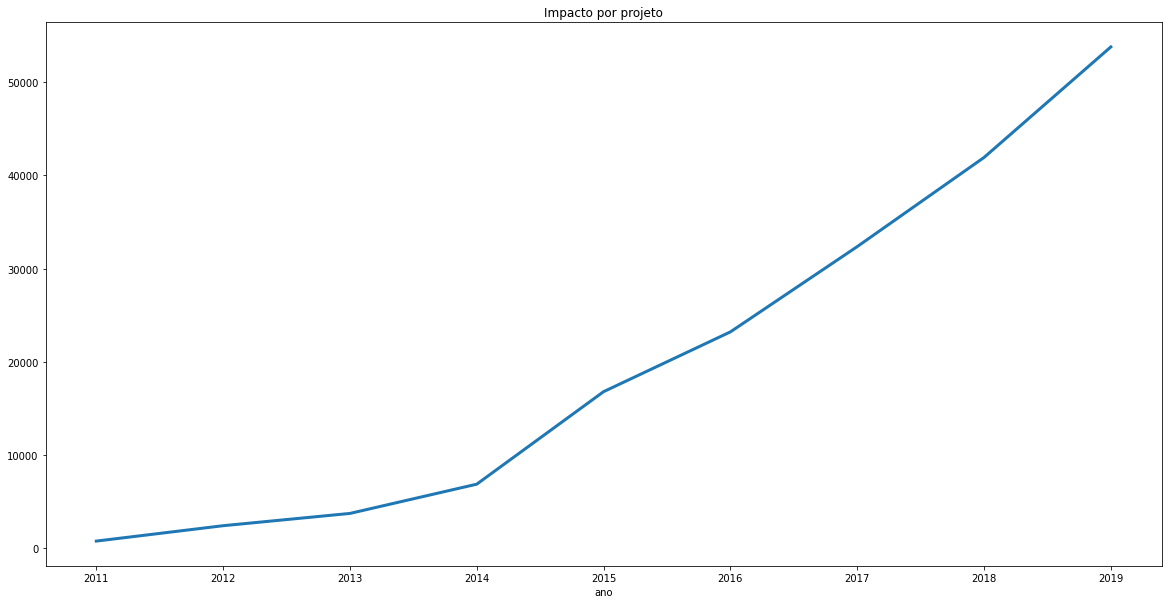
\includegraphics[width=1\textwidth]{Figuras/impactoanoTotal.png}
\caption{Número de estudantes possivelmente impactados por ano}
\label{fig:impactoAnoTotal}
\end{figure}




Já a Figura \ref{fig:idadeProjetos} apresenta o número de estudantes possivelmente impactados por sexo e idade de todos os projetos iniciados até 2019. É possível identificar a partir desta divisão por sexo que a média de idade das mulheres é levemente superior do que a idade dos homens, sendo aproximadamente 24,71 anos para a média feminina e 24,47 anos para os homens, que pode ser considerada igual. Já a mediana para ambos os sexos é de 23 anos. O pico das idades apresentam-se em 21 e 22 anos para ambos os sexos também.


\begin{figure}[H]
\centering
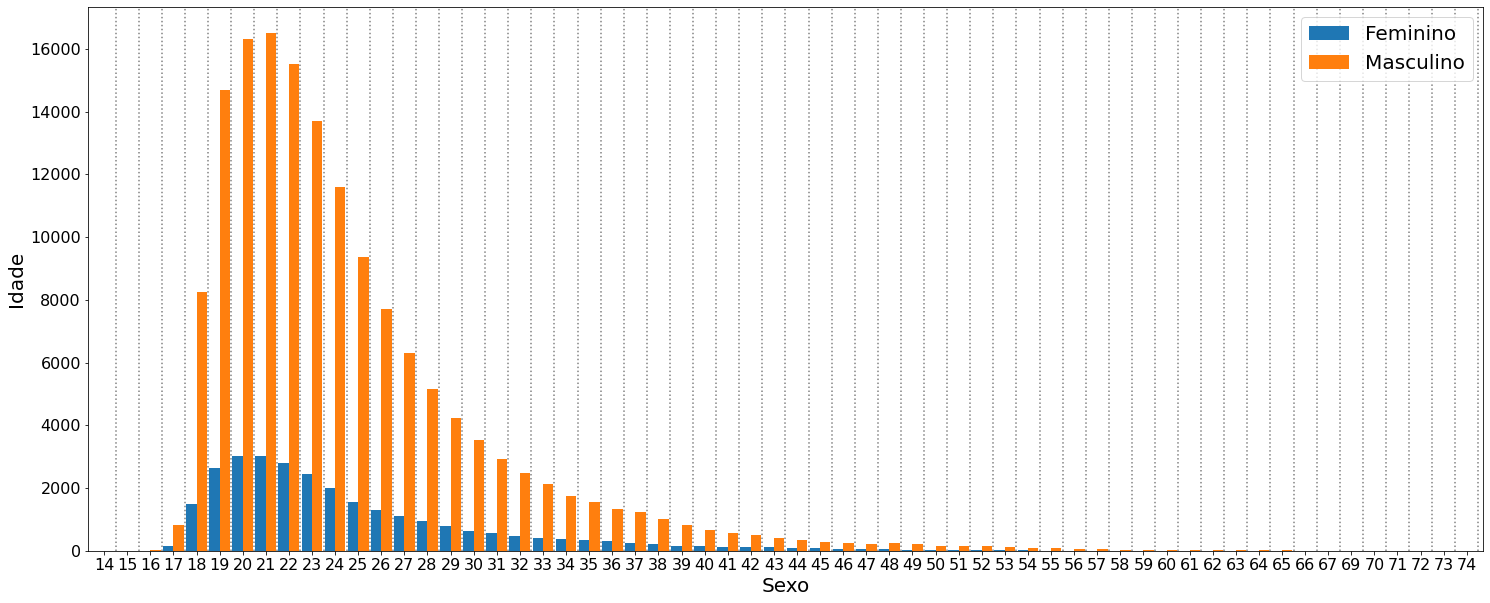
\includegraphics[width=1\textwidth]{Figuras/idadeProjetos.png}
\caption{Número de esetudantes possivelmente impactados categorizados por idade}
\label{fig:idadeProjetos}
\end{figure}








%\subsection{Projetos ativos}\label{sec:ProjetosAtivos}
%Após o levantamento dos projetos ativos, disponíveis no site Meninas Digitais, fez-se uma consulta ao comitê do programa para verificar os projetos ativos de fato, ou seja, os projetos que responderam ao questionário de participação ativa no ano de 2021. Chegando assim em um total de 72 projetos, que segundo a análise feita na Subseção \ref{sec:ProjetosLevantados} afeta então XX dos cursos XXXXXX (NOME DOS CURSOS 06 CINE).


\section{Projetos selecionados}\label{sec:ProjetosEscolhidos}

Por conta da pluralidade de projetos, foram selecionados 5 projetos a partir do possível impacto de cada um para exploração aprofundada. O impacto se dá pelo número de estudantes associados aos cursos e estudantes possivelmente afetados, com isso o gráfico da Figura \ref{fig:impactoProjetoTotal} explicita estes 5 projetos do programa Meninas Digitais. São eles WoMakersCode, Cunhantã Digital, Meninas Digitais Regional Sul, Meninas.Comp - Computação também é coisa de menina e Meninas Digitais Regional Mato Grosso do Sul.


% Please add the following required packages to your document preamble:
% \usepackage{multirow}
% \usepackage{graphicx}
% \usepackage[table,xcdraw]{xcolor}
% If you use beamer only pass "xcolor=table" option, i.e. \documentclass[xcolor=table]{beamer}
% \usepackage[normalem]{ulem}
% \useunder{\uline}{\ul}{}

% Please add the following required packages to your document preamble:
% \usepackage{multirow}
% \usepackage{graphicx}
% \usepackage[table,xcdraw]{xcolor}
% If you use beamer only pass "xcolor=table" option, i.e. \documentclass[xcolor=table]{beamer}
% \usepackage[normalem]{ulem}
% \useunder{\uline}{\ul}{}
\begin{table}[H]
\centering
\caption{Possível impacto por projetos selecionados}
\label{tab:ProjetosEscolhidos}
\resizebox{\textwidth}{!}{%
\begin{tabular}{|c|c|ccc|c|}
\hline
\rowcolor[HTML]{C0C0C0} 
\cellcolor[HTML]{C0C0C0}                     & \cellcolor[HTML]{C0C0C0}                                        & \multicolumn{3}{c|}{\cellcolor[HTML]{C0C0C0}Estudantes Possivelmente Impactados}                                    & \cellcolor[HTML]{C0C0C0}                         \\ \cline{3-5}
\rowcolor[HTML]{C0C0C0} 
\multirow{-2}{*}{\cellcolor[HTML]{C0C0C0}ID} & \multirow{-2}{*}{\cellcolor[HTML]{C0C0C0}Projetos Selecionados} & \multicolumn{1}{c|}{\cellcolor[HTML]{C0C0C0}Homens} & \multicolumn{1}{c|}{\cellcolor[HTML]{C0C0C0}Mulheres} & Total & \multirow{-2}{*}{\cellcolor[HTML]{C0C0C0}Início} \\ \hline
1                                            & WoMakersCode                                                    & \multicolumn{1}{c|}{12542}                          & \multicolumn{1}{c|}{1509}                             & 14051 & 2015                                             \\ \hline
2                                            & Cunhatã Digital                                                 & \multicolumn{1}{c|}{11017}                          & \multicolumn{1}{c|}{2488}                             & 13505 & 2015                                             \\ \hline
3                                            & Meninas Digitais Regional Sul                                   & \multicolumn{1}{c|}{10578}                          & \multicolumn{1}{c|}{1749}                             & 12327 & 2012                                             \\ \hline
4                                            & Meninas.Comp                                                    & \multicolumn{1}{c|}{9540}                           & \multicolumn{1}{c|}{1306}                             & 10846 & 2011                                             \\ \hline
5                                            & Meninas Digitais Regional Mato Grosso                           & \multicolumn{1}{c|}{7712}                           & \multicolumn{1}{c|}{3060}                             & 10772 & 2015                                             \\ \hline
\end{tabular}%
}
\end{table}



Dos 5 projetos escolhidos, cada um consecutivamente possivelmente afetam 7, 11, 3,3,3 cursos de TIC. A coluna ID da Tabela \ref{tab:ProjetosEscolhidosComCurso} relaciona-se com a coluna ID da Tabela \ref{fig:impactoProjetoTotal} para identificação de cada projeto. Os cursos, IES e seus códigos são apresentados na Tabela \ref{tab:ProjetosEscolhidosComCurso}.

\begin{longtable}[c]{|c|c|c|c|c|}
\caption{Cursos e IES relacionadas com os projetos selecionados}
\label{tab:ProjetosEscolhidosComCurso}\\
\hline
\rowcolor[HTML]{C0C0C0} 
\textbf{ID}          & \textbf{Código IES}    & \textbf{Nome IES}                                                                                                                  & \textbf{Código Curso}    & \textbf{Nome Curso}                                                                \\ \hline
\endfirsthead
%
\multicolumn{5}{c}%
{{\bfseries Tabela \thetable\ continuação da página anterior}} \\
\hline
\rowcolor[HTML]{C0C0C0} 
\textbf{ID}          & \textbf{Código IES}    & \textbf{Nome IES}                                                                                                                  & \textbf{Código Curso}    & \textbf{Nome Curso}                                                                \\ \hline
\endhead
%
                     &                        &                                                                                                                                    & 1904                     & Ciência da Computação                                                              \\ \cline{4-5} 
                     &                        &                                                                                                                                    & 56702                    & Engenharia da Computação                                                           \\ \cline{4-5} 
                     &                        &                                                                                                                                    & 56766                    & Sistemas de Informação                                                             \\ \cline{4-5} 
                     & \multirow{-4}{*}{21}   & \multirow{-4}{*}{\begin{tabular}[c]{@{}c@{}}Pontifícia \\ Universidade Católica\\  do Rio Grande do Sul\end{tabular}}              & 1314299                  & Engenharia de Software                                                             \\ \cline{2-5} 
                     &                        &                                                                                                                                    & 83904                    & \begin{tabular}[c]{@{}c@{}}Engenharia de Computação \\ e Informação\end{tabular}   \\ \cline{4-5} 
                     & \multirow{-2}{*}{586}  & \multirow{-2}{*}{\begin{tabular}[c]{@{}c@{}}Universidade Federal \\ do Rio de Janeiro\end{tabular}}                                & 85783                    & Ciência da Computação                                                              \\ \cline{2-5} 
\multirow{-7}{*}{1}  & 2950                   & \begin{tabular}[c]{@{}c@{}}Centro Universitário \\ FADERGS\end{tabular}                                                            & 1282899                  & Ciência da Computação                                                              \\ \hline
                     &                        &                                                                                                                                    & 62484                    & Ciência da Computação                                                              \\ \cline{4-5} 
                     &                        &                                                                                                                                    & 112086                   & Sistemas de Informação                                                             \\ \cline{4-5} 
                     &                        &                                                                                                                                    & 122634                   & Engenharia de Software                                                             \\ \cline{4-5} 
                     & \multirow{-4}{*}{4}    & \multirow{-4}{*}{\begin{tabular}[c]{@{}c@{}}Universidade Federal \\ do Amazonas\end{tabular}}                                      & 1158678                  & Engenharia de Software                                                             \\ \cline{2-5} 
                     &                        &                                                                                                                                    & 17886                    & Sistemas de Informação                                                             \\ \cline{4-5} 
                     &                        &                                                                                                                                    & 22061                    & Ciência da Computação                                                              \\ \cline{4-5} 
                     &                        &                                                                                                                                    & 110564                   & Engenharia de Computação                                                           \\ \cline{4-5} 
                     & \multirow{-4}{*}{1049} & \multirow{-4}{*}{\begin{tabular}[c]{@{}c@{}}Instituto de Ensino \\ Superior FUCAPI\end{tabular}}                                   & 1261039                  & Engenharia de Software                                                             \\ \cline{2-5} 
                     &                        &                                                                                                                                    & 69318                    & \begin{tabular}[c]{@{}c@{}}Análise e Desenvolvimento\\ de Sistemas\end{tabular}    \\ \cline{4-5} 
                     &                        &                                                                                                                                    & 1330347                  & Sistemas de Informação                                                             \\ \cline{4-5} 
\multirow{-11}{*}{2} & \multirow{-3}{*}{3172} & \multirow{-3}{*}{\begin{tabular}[c]{@{}c@{}}Universidade do Estado\\ do Amazonas\end{tabular}}                                     & 1330348                  & Jogos Digitais                                                                     \\ \hline
                     &                        &                                                                                                                                    & 14217                    & Ciência da Computação                                                              \\ \cline{4-5} 
                     &                        &                                                                                                                                    & 21600                    & Sistemas de Informação                                                             \\ \cline{4-5} 
\multirow{-1}{*}{3}  & \multirow{-1}{*}{585}  & \multirow{-1.5}{*}{\begin{tabular}[c]{@{}c@{}}Universidade Federal\\ de Santa Catarina\end{tabular}}                                 & 1084054                  & \begin{tabular}[c]{@{}c@{}}Tecnologias da Informação\\  e Comunicação\end{tabular} \\ \hline
                     &                        &                                                                                                                                    & 127                      & Ciência da Computação                                                              \\ \cline{4-5} 
                     &                        &                                                                                                                                    & 112891                   & Engenharia de Software                                                             \\ \cline{4-5} 
\multirow{-3}{*}{4}  & \multirow{-3}{*}{2}    & \multirow{-3}{*}{\begin{tabular}[c]{@{}c@{}}Universidade \\ de Brasília\end{tabular}}                                              & 122204                   & Engenharia de Computação                                                           \\ \hline
                     &                        &                                                                                                                                    & 65473                    & Sistemas para Internet                                                             \\ \cline{4-5} 
                     &                        &                                                                                                                                    & 90361                    & Redes de Computadores                                                              \\ \cline{4-5} 
                     &                        &                                                                                                                                    &                          &                                                                                    \\
\multirow{-4}{*}{5}  & \multirow{-4}{*}{3164} & \multirow{-4}{*}{\begin{tabular}[c]{@{}c@{}}Instituto Federal\\ de Educação, Ciência\\ e Tecnologia de\\ Mato Grosso\end{tabular}} & \multirow{-2}{*}{100694} & \multirow{-2}{*}{Sistemas para Internet}                                           \\ \hline
\end{longtable}

%Como todos os projetos presentes no site levantados tiveram sua última atualização no ano de 2020, decidiu-se por contatar o Programa Meninas Digitais e com isso uma tabela mais atual contendo apenas os projetos ativos no ano de 2022 com nome do projeto, cidade e ano de início foi disponibilizada e podem ser identificados pelas linhas coloridas da Tabela \ref{tab:ProjetosMeninasDigitais}. Alguns projetos disponíveis nesta planilha não constavam no site no dia da busca, por isso não foram considerados para esta pesquisa, são eles AI Girls - São Paulo (2020), IT Girls - Rio Tinto (2015), Meninas++ - Rio Paranaíba (2012), Minatech - Florianópolis (2021) e Projeto ADAs - Goiânia (2017). Apesar disso, os 5 projetos que possivelmente mais impactam pessoas não modificam-se, pois todos eram de fato projetos ativos e estavam contidos nessa atualização.

Com os projetos apresentados na Tabela \ref{tab:ProjetosEscolhidosComCurso} análises mais individuais são propostas na Seção \ref{sec:Avaliacoes} para entendimento da evasão no contexto desses projetos. 

\section{Análises}\label{sec:Avaliacoes}

As análises presentes nessa seção utilizam-se apenas dos dados do INEP relativos aos 5 projetos e aos 27 cursos que relacionam-se com tais projetos, descritos na Tabela \ref{tab:ProjetosEscolhidosComCurso}.

As Figuras \ref{fig:calorCorRaca}, \ref{fig:calorFormaIngresso} e \ref{fig:calorIdade} são gráficos de calor com a evolução anual da evasão de acordo com os parâmetros de cor e raça, forma de ingresso e idade dos estudantes possivelmente envolvidos nos projetos selecionados.
É importante neste ponto relembrar que a Equação utilizada para o cálculo da evasão está disponível na Seção \ref{sec:CalculoEvasao}.


As análises apresentadas foram feitas a partir de dados fornecidos pelo INEP. Todas as análises baseiam-se na divisão de gênero disponível no banco de dados, as variáveis mostradas são apenas feminino e masculino, bem como todas as outras divisões de cor e raça e forma de ingresso.

INÍCIO ANÁLISES NOVAS:

\begin{figure}[H]
\centering
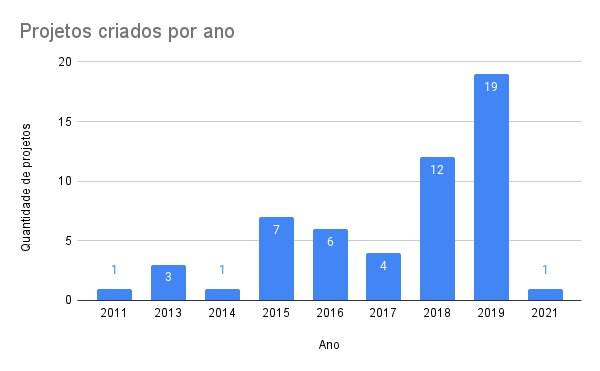
\includegraphics[width=1\textwidth]{Figuras/ProjetosPorAno.jpeg}
\caption{---}
\label{fig:ProjetosPorAno}
\end{figure}
 
\begin{figure}[H]
\centering
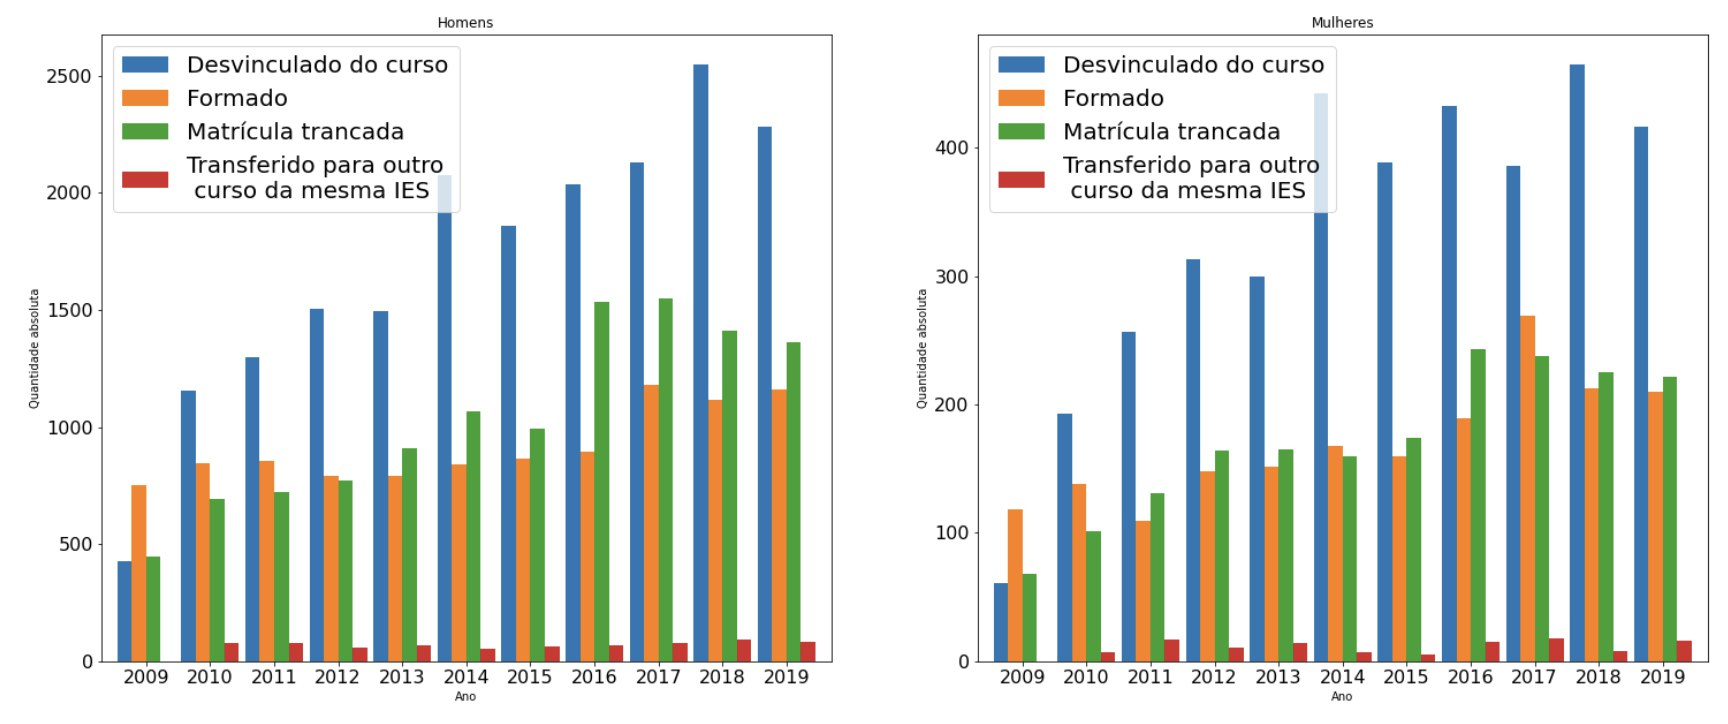
\includegraphics[width=1\textwidth]{Figuras/situacaodosalunos.jpeg}
\caption{---}
\label{fig:situacaodosalunos}
\end{figure}

\begin{figure}[H]
\centering
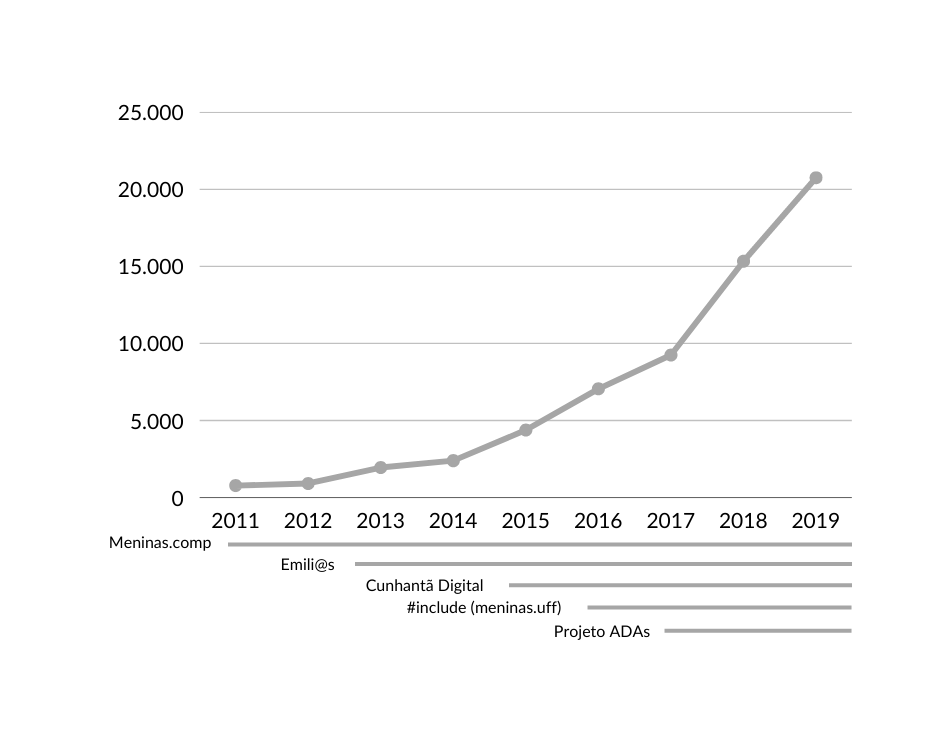
\includegraphics[width=1\textwidth]{Figuras/numeroalunosprojeto.png}
\caption{---}
\label{fig:numeroalunosprojeto}
\end{figure}


\begin{figure}[H]
\centering
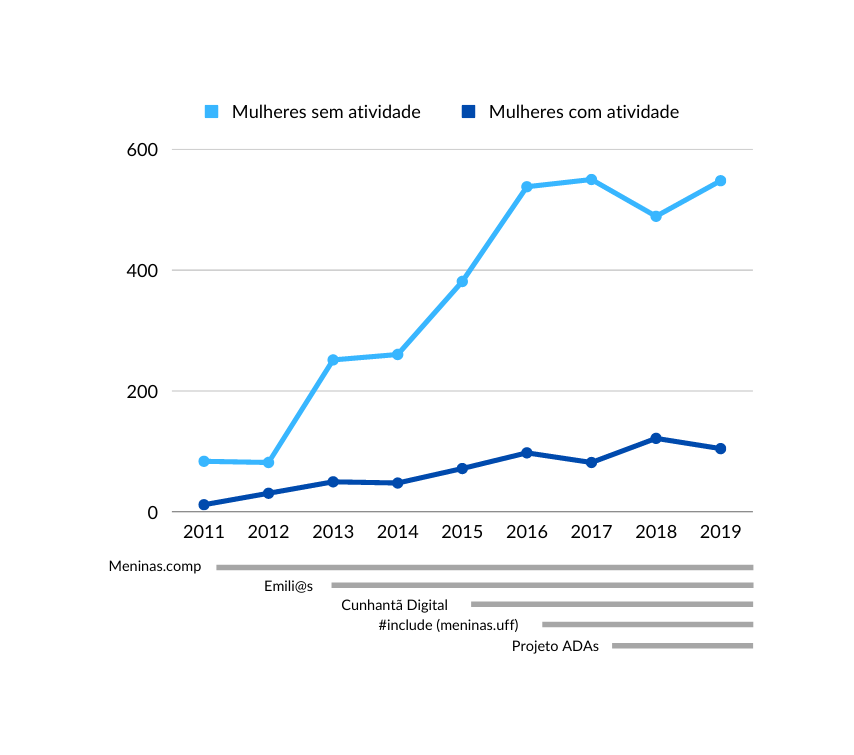
\includegraphics[width=1\textwidth]{Figuras/atividadeextra.png}
\caption{---}
\label{fig:atividadeextra}
\end{figure}


\begin{figure}[H]
\centering
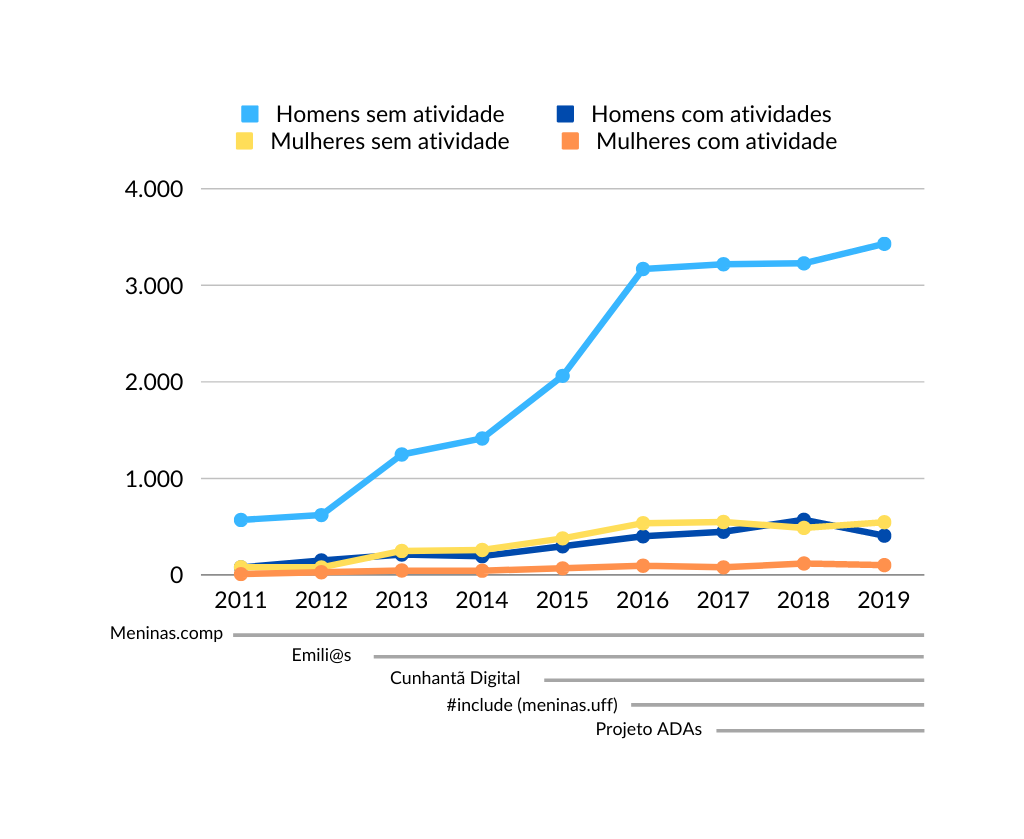
\includegraphics[width=1\textwidth]{Figuras/quantidadeatividadeextra.png}
\caption{---}
\label{fig:quantidadeatividadeextra}
\end{figure}


FIM ANÁLISES NOVAS


\subsection{Evasão por Ano, Cor e Raça}\label{sub:calorCorERaca}
A Figura \ref{fig:calorCorRaca} apresenta as informações quanto ao gênero, raça e taxa de evasão. Percebe-se que a evasão máxima em porcentagem acontece no ano de 2012 onde 75\% das mulheres que não quiseram declarar sua cor e raça evadiram. Embora preocupante, esse valor é atrelado a baixa quantidade de mulheres pertencentes a esse grupo.

Além disso, há vários pontos onde a taxa de evasão é zerada, significando que, dos estudantes evadidos daquele período, nenhum pertencia ao determinado grupo. Vale ressaltar que alguns campos estão sem informações pois não haviam estudantes nesse grupo e período.


\begin{figure}[H]
\centering
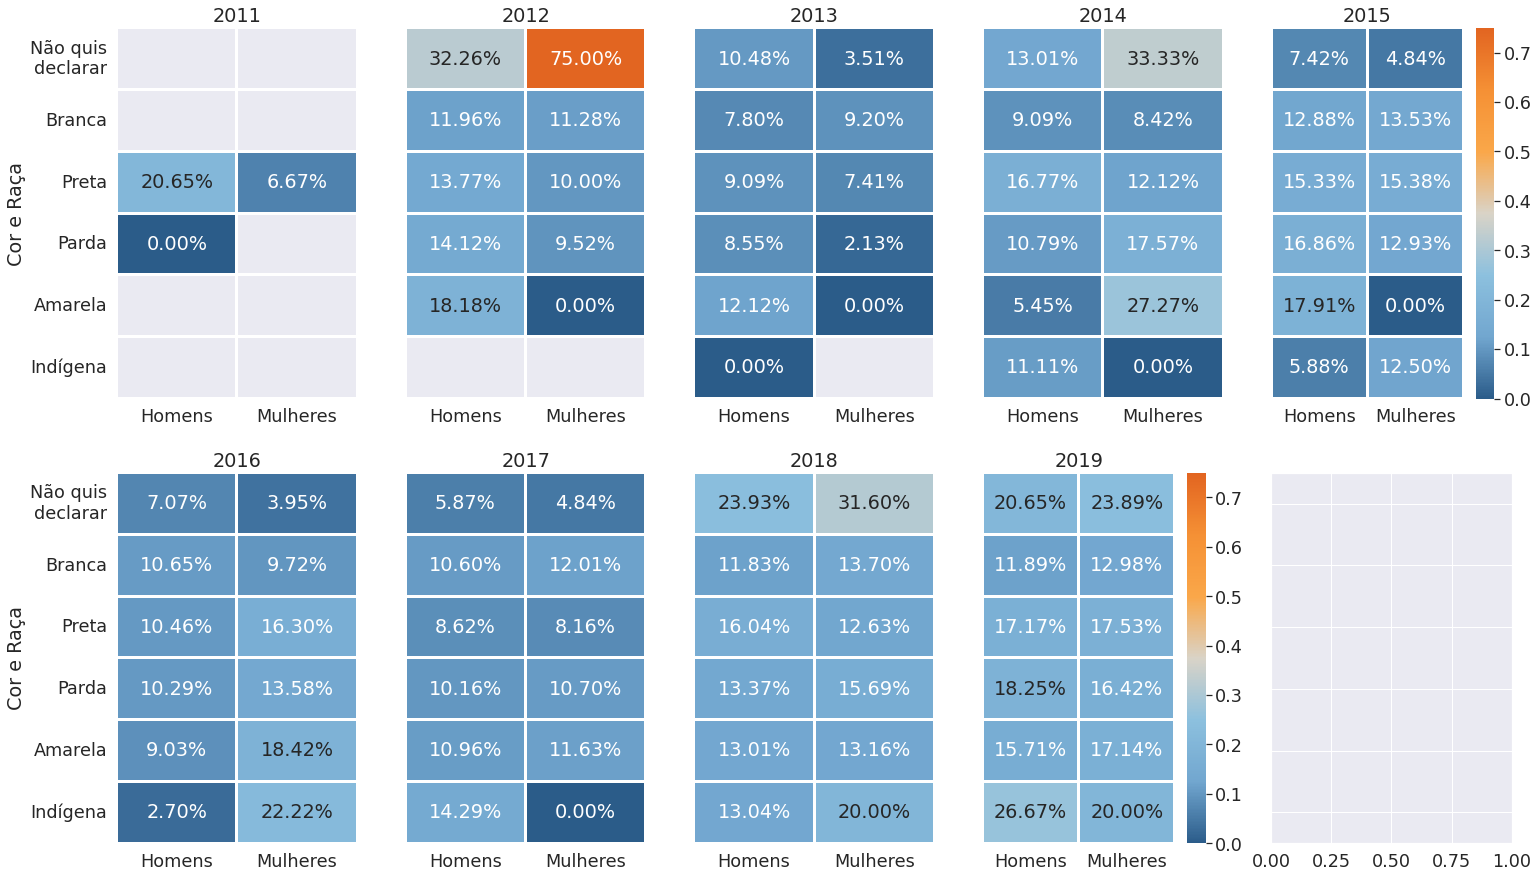
\includegraphics[width=1\textwidth]{Figuras/calorCorRaca.png}
\caption{Evasão do conjunto de projetos selecionados por ano, cor e raça}
\label{fig:calorCorRaca}
\end{figure}

No decorrer de todos os anos nenhum dos grupos apresentou alta contínua ou queda continua, mas é interessante observar o comportamento das indígenas, que variam entre zero e aproximadamente 20\% de um ano para outro, reforçando que o número de mulheres indígenas é baixo e com apenas uma evasão a taxa sobe significativamente.

Apesar de nenhum grupo apresentar queda ou crescente contínua para todos os anos, todos os grupos apresentam queda no ano de 2012 para 2013. De 2015 a 2016 todos os homens apresentaram queda na taxa de evasão e apenas as mulheres que não quiseram declarar e as brancas seguiram esta tendência, o restante do grupo teve um aumento na taxa de evasão.

Em uma visão com valores absolutos apresentadas nas Tabelas \ref{tab:numabsoluto2011}, \ref{tab:numabsoluto2014} e \ref{tab:numabsoluto2017} onde observa-se que em nenhum dos grupos o número de homens é inferior ao número de mulheres. Lembrando que os valores absolutos de estudantes não trazem uma relação direta com a evasão, pois por exemplo, o número de estudantes mulheres amarelas pode ter permanecido o mesmo em dois anos distintos ou até aumentado, mas todas as mulheres do ano X podem ter evadido em X+1 e X+1 pode apresentar mulheres distintas ingressantes, tendo assim uma taxa de evasão elevada.


\begin{table}[H]
\caption{Número absoluto de estudantes por ano, gênero, cor e raça de 2011 a 2013}
\label{tab:numabsoluto2011}
\resizebox{\textwidth}{!}{%
\begin{tabular}{c|cc|cc|cc|}
\cline{2-7}
                                                                         & \multicolumn{2}{c|}{\cellcolor[HTML]{C0C0C0}\textbf{2011}}                                               & \multicolumn{2}{c|}{\cellcolor[HTML]{C0C0C0}\textbf{2012}}                                               & \multicolumn{2}{c|}{\cellcolor[HTML]{C0C0C0}\textbf{2013}}                                               \\ \cline{2-7} 
\multirow{-2}{*}{}                                                       & \multicolumn{1}{c|}{\cellcolor[HTML]{C0C0C0}\textbf{Homens}} & \cellcolor[HTML]{C0C0C0}\textbf{Mulheres} & \multicolumn{1}{c|}{\cellcolor[HTML]{C0C0C0}\textbf{Homens}} & \cellcolor[HTML]{C0C0C0}\textbf{Mulheres} & \multicolumn{1}{c|}{\cellcolor[HTML]{C0C0C0}\textbf{Homens}} & \cellcolor[HTML]{C0C0C0}\textbf{Mulheres} \\ \hline
\multicolumn{1}{|c|}{\cellcolor[HTML]{C0C0C0}\textbf{Não quis declarar}} & \multicolumn{1}{c|}{0}                                       & 0                                         & \multicolumn{1}{c|}{31}                                      & 4                                         & \multicolumn{1}{c|}{301}                                     & 54                                        \\ \hline
\multicolumn{1}{|c|}{\cellcolor[HTML]{C0C0C0}\textbf{Branca}}            & \multicolumn{1}{c|}{0}                                       & 0                                         & \multicolumn{1}{c|}{1129}                                    & 195                                       & \multicolumn{1}{c|}{1389}                                    & 220                                       \\ \hline
\multicolumn{1}{|c|}{\cellcolor[HTML]{C0C0C0}\textbf{Preta}}             & \multicolumn{1}{c|}{92}                                      & 15                                        & \multicolumn{1}{c|}{143}                                     & 28                                        & \multicolumn{1}{c|}{104}                                     & 23                                        \\ \hline
\multicolumn{1}{|c|}{\cellcolor[HTML]{C0C0C0}\textbf{Parda}}             & \multicolumn{1}{c|}{1}                                       & 0                                         & \multicolumn{1}{c|}{85}                                      & 21                                        & \multicolumn{1}{c|}{249}                                     & 45                                        \\ \hline
\multicolumn{1}{|c|}{\cellcolor[HTML]{C0C0C0}\textbf{Amarela}}           & \multicolumn{1}{c|}{0}                                       & 0                                         & \multicolumn{1}{c|}{11}                                      & 2                                         & \multicolumn{1}{c|}{29}                                      & 8                                         \\ \hline
\multicolumn{1}{|c|}{\cellcolor[HTML]{C0C0C0}\textbf{Indígena}}          & \multicolumn{1}{c|}{0}                                       & 0                                         & \multicolumn{1}{c|}{0}                                       & 0                                         & \multicolumn{1}{c|}{1}                                       & 0                                         \\ \hline
\end{tabular}%
}
\end{table}

\begin{table}[H]
\caption{Número absoluto de estudantes por ano, gênero, cor e raça de 2014 a 2016}
\label{tab:numabsoluto2014}
\resizebox{\textwidth}{!}{%
\begin{tabular}{c|cc|cc|cc|}
\cline{2-7}
                                                                         & \multicolumn{2}{c|}{\cellcolor[HTML]{C0C0C0}\textbf{2014}}                                               & \multicolumn{2}{c|}{\cellcolor[HTML]{C0C0C0}\textbf{2015}}                                               & \multicolumn{2}{c|}{\cellcolor[HTML]{C0C0C0}\textbf{2016}}                                               \\ \cline{2-7} 
\multirow{-2}{*}{}                                                       & \multicolumn{1}{c|}{\cellcolor[HTML]{C0C0C0}\textbf{Homens}} & \cellcolor[HTML]{C0C0C0}\textbf{Mulheres} & \multicolumn{1}{c|}{\cellcolor[HTML]{C0C0C0}\textbf{Homens}} & \cellcolor[HTML]{C0C0C0}\textbf{Mulheres} & \multicolumn{1}{c|}{\cellcolor[HTML]{C0C0C0}\textbf{Homens}} & \cellcolor[HTML]{C0C0C0}\textbf{Mulheres} \\ \hline
\multicolumn{1}{|c|}{\cellcolor[HTML]{C0C0C0}\textbf{Não quis declarar}} & \multicolumn{1}{c|}{96}                                      & 15                                        & \multicolumn{1}{c|}{1362}                                    & 489                                       & \multicolumn{1}{c|}{1280}                                    & 475                                       \\ \hline
\multicolumn{1}{|c|}{\cellcolor[HTML]{C0C0C0}\textbf{Branca}}            & \multicolumn{1}{c|}{1601}                                    & 254                                       & \multicolumn{1}{c|}{4265}                                    & 649                                       & \multicolumn{1}{c|}{4324}                                    & 634                                       \\ \hline
\multicolumn{1}{|c|}{\cellcolor[HTML]{C0C0C0}\textbf{Preta}}             & \multicolumn{1}{c|}{145}                                     & 31                                        & \multicolumn{1}{c|}{364}                                     & 70                                        & \multicolumn{1}{c|}{399}                                     & 75                                        \\ \hline
\multicolumn{1}{|c|}{\cellcolor[HTML]{C0C0C0}\textbf{Parda}}             & \multicolumn{1}{c|}{382}                                     & 72                                        & \multicolumn{1}{c|}{2202}                                    & 511                                       & \multicolumn{1}{c|}{2328}                                    & 508                                       \\ \hline
\multicolumn{1}{|c|}{\cellcolor[HTML]{C0C0C0}\textbf{Amarela}}           & \multicolumn{1}{c|}{49}                                      & 11                                        & \multicolumn{1}{c|}{129}                                     & 31                                        & \multicolumn{1}{c|}{113}                                     & 37                                        \\ \hline
\multicolumn{1}{|c|}{\cellcolor[HTML]{C0C0C0}\textbf{Indígena}}          & \multicolumn{1}{c|}{9}                                       & 2                                         & \multicolumn{1}{c|}{31}                                      & 7                                         & \multicolumn{1}{c|}{30}                                      & 8                                         \\ \hline
\end{tabular}%
}
\end{table}

\begin{table}[H]
\caption{Número absoluto de estudantes por ano, gênero, cor e raça de 2017 a 2019}
\label{tab:numabsoluto2017}
\resizebox{\textwidth}{!}{%
\begin{tabular}{c|cc|cc|cc|}
\cline{2-7}
                                                                         & \multicolumn{2}{c|}{\cellcolor[HTML]{C0C0C0}\textbf{2017}}                                               & \multicolumn{2}{c|}{\cellcolor[HTML]{C0C0C0}\textbf{2018}}                                               & \multicolumn{2}{c|}{\cellcolor[HTML]{C0C0C0}\textbf{2019}}                                               \\ \cline{2-7} 
\multirow{-2}{*}{}                                                       & \multicolumn{1}{c|}{\cellcolor[HTML]{C0C0C0}\textbf{Homens}} & \cellcolor[HTML]{C0C0C0}\textbf{Mulheres} & \multicolumn{1}{c|}{\cellcolor[HTML]{C0C0C0}\textbf{Homens}} & \cellcolor[HTML]{C0C0C0}\textbf{Mulheres} & \multicolumn{1}{c|}{\cellcolor[HTML]{C0C0C0}\textbf{Homens}} & \cellcolor[HTML]{C0C0C0}\textbf{Mulheres} \\ \hline
\multicolumn{1}{|c|}{\cellcolor[HTML]{C0C0C0}\textbf{Não quis declarar}} & \multicolumn{1}{c|}{1600}                                    & 597                                       & \multicolumn{1}{c|}{1461}                                    & 513                                       & \multicolumn{1}{c|}{1109}                                    & 321                                       \\ \hline
\multicolumn{1}{|c|}{\cellcolor[HTML]{C0C0C0}\textbf{Branca}}            & \multicolumn{1}{c|}{4430}                                    & 656                                       & \multicolumn{1}{c|}{4400}                                    & 626                                       & \multicolumn{1}{c|}{4243}                                    & 604                                       \\ \hline
\multicolumn{1}{|c|}{\cellcolor[HTML]{C0C0C0}\textbf{Preta}}             & \multicolumn{1}{c|}{458}                                     & 81                                        & \multicolumn{1}{c|}{471}                                     & 80                                        & \multicolumn{1}{c|}{452}                                     & 81                                        \\ \hline
\multicolumn{1}{|c|}{\cellcolor[HTML]{C0C0C0}\textbf{Parda}}             & \multicolumn{1}{c|}{2569}                                    & 542                                       & \multicolumn{1}{c|}{2704}                                    & 568                                       & \multicolumn{1}{c|}{2658}                                    & 549                                       \\ \hline
\multicolumn{1}{|c|}{\cellcolor[HTML]{C0C0C0}\textbf{Amarela}}           & \multicolumn{1}{c|}{125}                                     & 34                                        & \multicolumn{1}{c|}{123}                                     & 28                                        & \multicolumn{1}{c|}{109}                                     & 29                                        \\ \hline
\multicolumn{1}{|c|}{\cellcolor[HTML]{C0C0C0}\textbf{Indígena}}          & \multicolumn{1}{c|}{39}                                      & 6                                         & \multicolumn{1}{c|}{38}                                      & 5                                         & \multicolumn{1}{c|}{38}                                      & 4                                         \\ \hline
\end{tabular}%
}
\end{table}


\subsection{Evasão por Ano e Forma de Ingresso}\label{sub:calorFomaIngresso}

Para a apresentação do gráfico da Figura \ref{fig:calorFormaIngresso}, as categorias não nulas presentes na base de dados são referentes a forma com que o estudante ingressou na IES e são identificadas por:
\begin{itemize}
    \item Enem: Informa se o estudante ingressou no curso pelo Enem;
    \item Ensino Público:  Informa se o estudante ingressou por meio de programa de reserva de vagas para egressos da escola pública;
    \item Renda Familiar: Informa se o estudante ingressou por meio de programa de reserva de vagas de cunho social ou de renda familiar;
    \item Reserva de Vagas: Informa se o estudante participa de programa de reserva de vagas;
    \item Seleção Simplificada: Informa se o estudante ingressou no curso por meio de seleção simplificada;
    \item Vagas Remanescentes: Informa se o estudante ingressou no curso por meio de vagas remanescentes;
    \item Vagas Étnicas: Informa se o estudante ingressou por meio de programa de reserva de vagas de cunho étnico;
    \item Vestibular: Informa se o estudante ingressou no curso pelo vestibular.
\end{itemize}

A análise das formas de ingresso nas instituições citadas presente na Figura \ref{fig:calorFormaIngresso}, relacionando-se com gênero e taxa de evasão por ano, desde 2011 até 2019. O ponto onde o gráfico possui a maior taxa de evasão pertence ao ano de 2014, onde, dos homens que ingressaram pelo programa de renda familiar, 33,33\% evadiram. Já com as estudantes mulheres, a maior porcentagem está no ano de 2018 onde 26,09\% que ingressaram pelo programa de seleção simplificada evadiram. 

\begin{figure}[H]
\centering
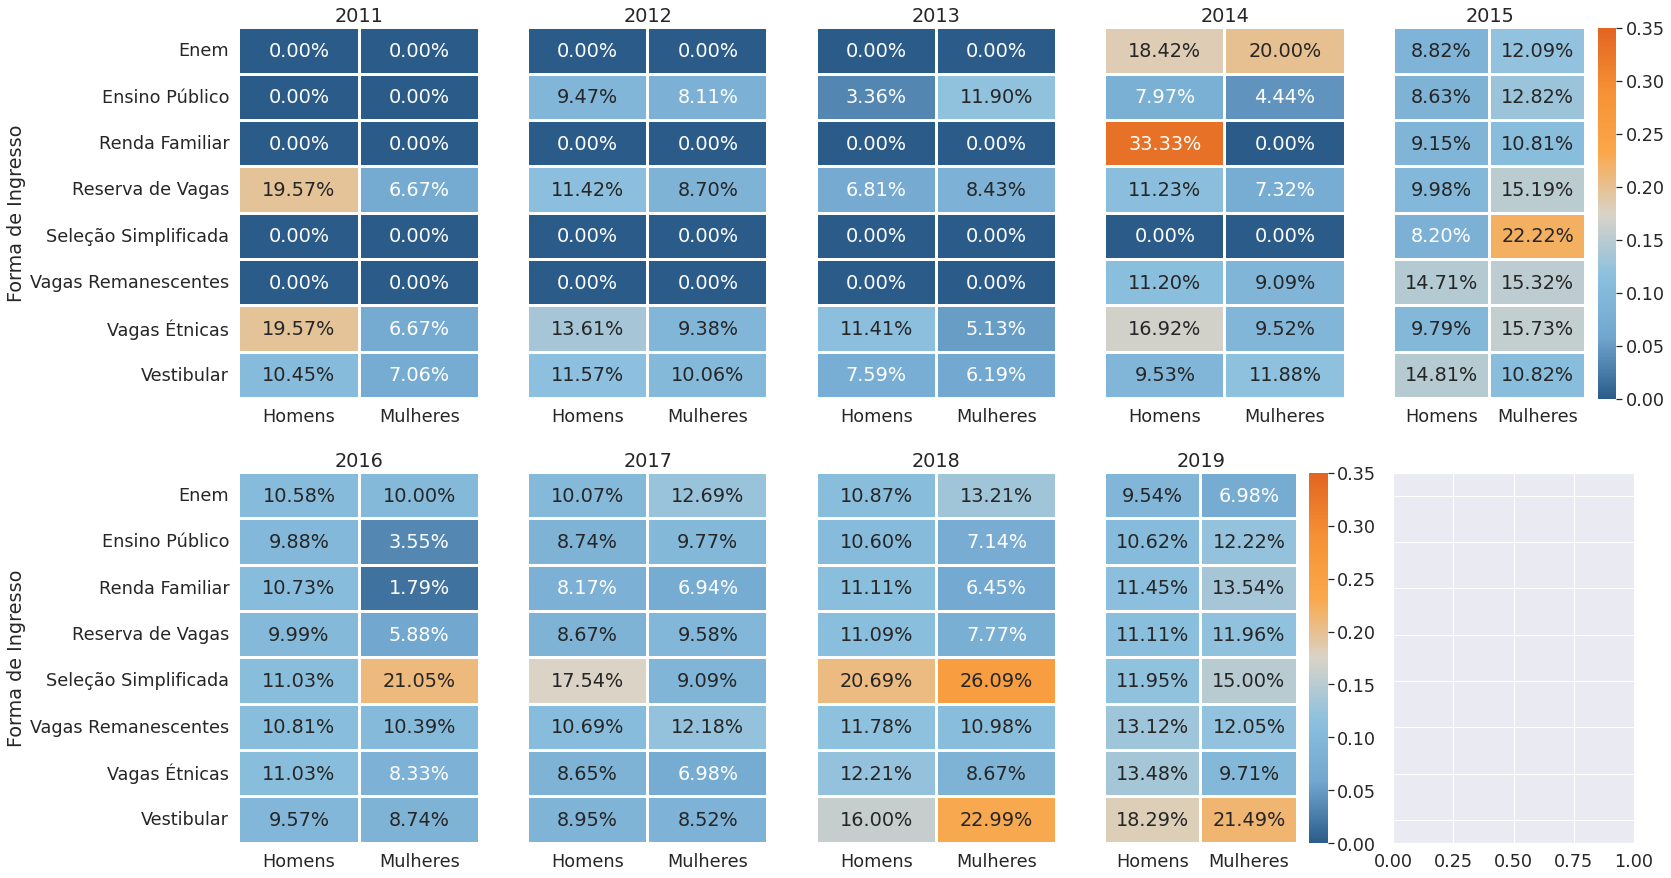
\includegraphics[width=1\textwidth]{Figuras/calorFormaIngresso.png}
\caption{Evasão do conjunto de projetos selecionados por ano e forma de ingresso}
\label{fig:calorFormaIngresso}
\end{figure}

É possível observar também que apresentam maior frequência de valores altos para da taxa de evasão as mulheres que ingressaram por seleção simplificada, onde inicialmente apresentavam taxa zero até o ano de 2014. Em números absolutos em ordem crescente de anos iniciando em 2011, o número de mulheres que ingressaram nas IES pela seleção simplificada foi 0, 0, 0, 0, 18, 15, 18, 20 e 14.

Também é possível observar todos os homens e mulheres que ingressaram por meio do vestibular e vagas étnicas entre os anos de 2017, 2018 e 2019 apresentaram alta na porcentagem de evasão.


\subsection{Evasão por Ano e Idade}\label{sub:calorIdade}
%COLOCAR ALGO ASSIM:
%No conjunto de dados observado, a diferença de idade máxima encontrada entre homens e mulheres foi bastante significativa, sendo 61 anos para homens e 48 anos para mulheres. Essa faixa etária, porém, é pouco presente no curso, que possui estudantes com uma idade média de 22 anos, tanto para homens quanto para mulheres. Portanto, considerando os dados anteriores, o intervalo de análise mínimo proposto foi de até 25 anos, com intervalo máximo de mais de 55 anos. 


A Figura \ref{fig:calorIdade} apresenta a relação entre gênero, idade e taxa de evasão nos anos observados. Um dos pontos críticos, onde houve maior evasão do gráfico ocorreu em 2012, em que, considerando apenas o número total de homens com idade maior de 55 anos, 66,67\% daqueles que estavam nessa faixa etária evadiram. Para mulheres, o ponto de máxima porcentagem ocorreu nos anos de 2013 e 2018, na faixa etária de maior de 55 anos, em que 50\% das mulheres contidas nessa faixa de idade evadiram. Observa-se nos extremos do gráfico, ou seja nas menores idades e maiores idades, um grande número de porcentagens zeradas, pois nessa faixa etária o número de estudantes mostra-se reduzido, fazendo com que cada estudante evadido tenha uma grande alta na porcentagem bem como quando nenhum estudante evade o que faz com que a taxa fique zerada.

Além disso, percebe-se que as menores taxas de evasão são de estudantes com faixa etária de até 25 anos. É importante pontuar que quadrados que não possuem a porcentagem de evasão e aparecem sem cor estão dessa forma pois nos anos analisados não haviam estudantes naquela faixa etária, e portanto não é possível concluir sobre a taxa de evasão para a mesma. 


\begin{figure}[H]
\centering
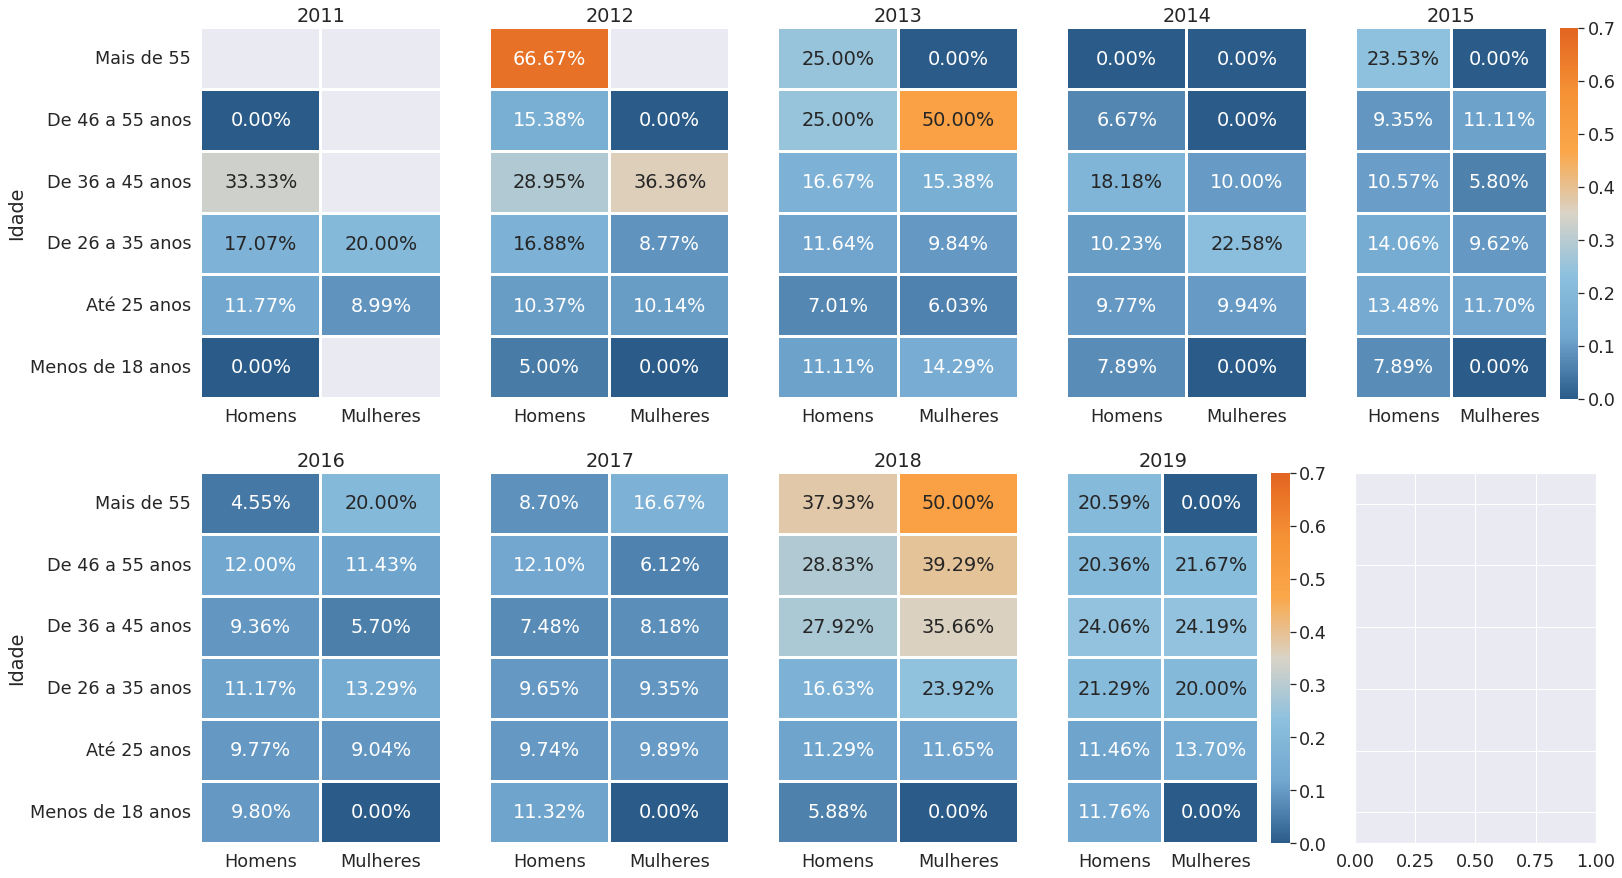
\includegraphics[width=1\textwidth]{Figuras/calorIdade.png}
\caption{Evasão do conjunto de projetos selecionados por ano e faixa etária}
\label{fig:calorIdade}
\end{figure}

As Tabelas \ref{tab:numabsoluto2011Idade}, \ref{tab:numabsoluto2014Idade} e \ref{tab:numabsoluto2017Idade} apresentam os valores absolutos de estudante dos anos de 2011 a 2019 por faixa etária.

\begin{table}[H]
\caption{Número absoluto de estudantes por ano, gênero e idade de 2011 a 2013}
\label{tab:numabsoluto2011Idade}
\resizebox{\textwidth}{!}{%
\begin{tabular}{c|cc|cc|cc|}
\cline{2-7}
                                                                        & \multicolumn{2}{c|}{\cellcolor[HTML]{C0C0C0}\textbf{2011}}                                               & \multicolumn{2}{c|}{\cellcolor[HTML]{C0C0C0}\textbf{2012}}                                               & \multicolumn{2}{c|}{\cellcolor[HTML]{C0C0C0}\textbf{2013}}                                               \\ \cline{2-7} 
\multirow{-2}{*}{}                                                      & \multicolumn{1}{c|}{\cellcolor[HTML]{C0C0C0}\textbf{Homens}} & \cellcolor[HTML]{C0C0C0}\textbf{Mulheres} & \multicolumn{1}{c|}{\cellcolor[HTML]{C0C0C0}\textbf{Homens}} & \cellcolor[HTML]{C0C0C0}\textbf{Mulheres} & \multicolumn{1}{c|}{\cellcolor[HTML]{C0C0C0}\textbf{Homens}} & \cellcolor[HTML]{C0C0C0}\textbf{Mulheres} \\ \hline
\multicolumn{1}{|c|}{\cellcolor[HTML]{C0C0C0}\textbf{Mais de 55 anos}}  & \multicolumn{1}{c|}{0}                                       & 0                                         & \multicolumn{1}{c|}{3}                                       & 0                                         & \multicolumn{1}{c|}{2}                                       & 1                                         \\ \hline
\multicolumn{1}{|c|}{\cellcolor[HTML]{C0C0C0}\textbf{De 46 a 55 anos}}  & \multicolumn{1}{c|}{2}                                       & 0                                         & \multicolumn{1}{c|}{13}                                      & 2                                         & \multicolumn{1}{c|}{14}                                      & 2                                         \\ \hline
\multicolumn{1}{|c|}{\cellcolor[HTML]{C0C0C0}\textbf{De 36 a 45 anos}}  & \multicolumn{1}{c|}{6}                                       & 0                                         & \multicolumn{1}{c|}{36}                                      & 11                                        & \multicolumn{1}{c|}{35}                                      & 9                                         \\ \hline
\multicolumn{1}{|c|}{\cellcolor[HTML]{C0C0C0}\textbf{De 26 a 35 anos}}  & \multicolumn{1}{c|}{41}                                      & 5                                         & \multicolumn{1}{c|}{370}                                     & 55                                        & \multicolumn{1}{c|}{367}                                     & 50                                        \\ \hline
\multicolumn{1}{|c|}{\cellcolor[HTML]{C0C0C0}\textbf{De 18 a 25 anos}}  & \multicolumn{1}{c|}{603}                                     & 89                                        & \multicolumn{1}{c|}{1634}                                    & 274                                       & \multicolumn{1}{c|}{1732}                                    & 302                                       \\ \hline
\multicolumn{1}{|c|}{\cellcolor[HTML]{C0C0C0}\textbf{Menos de 18 anos}} & \multicolumn{1}{c|}{0}                                       & 0                                         & \multicolumn{1}{c|}{16}                                      & 3                                         & \multicolumn{1}{c|}{33}                                      & 7                                         \\ \hline
\end{tabular}%
}
\end{table}

\begin{table}[H]
\caption{Número absoluto de estudantes por ano, gênero e idade de 2014 a 2016}
\label{tab:numabsoluto2014Idade}
\resizebox{\textwidth}{!}{%
\begin{tabular}{c|cc|cc|cc|}
\cline{2-7}
                                                                        & \multicolumn{2}{c|}{\cellcolor[HTML]{C0C0C0}\textbf{2014}}                                               & \multicolumn{2}{c|}{\cellcolor[HTML]{C0C0C0}\textbf{2015}}                                               & \multicolumn{2}{c|}{\cellcolor[HTML]{C0C0C0}\textbf{2016}}                                               \\ \cline{2-7} 
\multirow{-2}{*}{}                                                      & \multicolumn{1}{c|}{\cellcolor[HTML]{C0C0C0}\textbf{Homens}} & \cellcolor[HTML]{C0C0C0}\textbf{Mulheres} & \multicolumn{1}{c|}{\cellcolor[HTML]{C0C0C0}\textbf{Homens}} & \cellcolor[HTML]{C0C0C0}\textbf{Mulheres} & \multicolumn{1}{c|}{\cellcolor[HTML]{C0C0C0}\textbf{Homens}} & \cellcolor[HTML]{C0C0C0}\textbf{Mulheres} \\ \hline
\multicolumn{1}{|c|}{\cellcolor[HTML]{C0C0C0}\textbf{Mais de 55 anos}}  & \multicolumn{1}{c|}{2}                                       & 1                                         & \multicolumn{1}{c|}{17}                                      & 3                                         & \multicolumn{1}{c|}{17}                                      & 4                                         \\ \hline
\multicolumn{1}{|c|}{\cellcolor[HTML]{C0C0C0}\textbf{De 46 a 55 anos}}  & \multicolumn{1}{c|}{10}                                      & 2                                         & \multicolumn{1}{c|}{106}                                     & 27                                        & \multicolumn{1}{c|}{107}                                     & 32                                        \\ \hline
\multicolumn{1}{|c|}{\cellcolor[HTML]{C0C0C0}\textbf{De 36 a 45 anos}}  & \multicolumn{1}{c|}{35}                                      & 8                                         & \multicolumn{1}{c|}{442}                                     & 137                                       & \multicolumn{1}{c|}{476}                                     & 145                                       \\ \hline
\multicolumn{1}{|c|}{\cellcolor[HTML]{C0C0C0}\textbf{De 26 a 35 anos}}  & \multicolumn{1}{c|}{409}                                     & 46                                        & \multicolumn{1}{c|}{2314}                                    & 533                                       & \multicolumn{1}{c|}{2346}                                    & 544                                       \\ \hline
\multicolumn{1}{|c|}{\cellcolor[HTML]{C0C0C0}\textbf{De 18 a 25 anos}}  & \multicolumn{1}{c|}{1836}                                    & 329                                       & \multicolumn{1}{c|}{5674}                                    & 1110                                      & \multicolumn{1}{c|}{5646}                                    & 1051                                      \\ \hline
\multicolumn{1}{|c|}{\cellcolor[HTML]{C0C0C0}\textbf{Menos de 18 anos}} & \multicolumn{1}{c|}{35}                                      & 3                                         & \multicolumn{1}{c|}{33}                                      & 2                                         & \multicolumn{1}{c|}{45}                                      & 10                                        \\ \hline
\end{tabular}%
}
\end{table}

\begin{table}[H]
\caption{Número absoluto de estudantes por ano, gênero e idade de 2017 a 2019}
\label{tab:numabsoluto2017Idade}
\resizebox{\textwidth}{!}{%
\begin{tabular}{c|cc|cc|cc|}
\cline{2-7}
                                                                        & \multicolumn{2}{c|}{\cellcolor[HTML]{C0C0C0}\textbf{2017}}                                               & \multicolumn{2}{c|}{\cellcolor[HTML]{C0C0C0}\textbf{2018}}                                               & \multicolumn{2}{c|}{\cellcolor[HTML]{C0C0C0}\textbf{2019}}                                               \\ \cline{2-7} 
\multirow{-2}{*}{}                                                      & \multicolumn{1}{c|}{\cellcolor[HTML]{C0C0C0}\textbf{Homens}} & \cellcolor[HTML]{C0C0C0}\textbf{Mulheres} & \multicolumn{1}{c|}{\cellcolor[HTML]{C0C0C0}\textbf{Homens}} & \cellcolor[HTML]{C0C0C0}\textbf{Mulheres} & \multicolumn{1}{c|}{\cellcolor[HTML]{C0C0C0}\textbf{Homens}} & \cellcolor[HTML]{C0C0C0}\textbf{Mulheres} \\ \hline
\multicolumn{1}{|c|}{\cellcolor[HTML]{C0C0C0}\textbf{Mais de 55 anos}}  & \multicolumn{1}{c|}{22}                                      & 5                                         & \multicolumn{1}{c|}{26}                                      & 5                                         & \multicolumn{1}{c|}{22}                                      & 2                                         \\ \hline
\multicolumn{1}{|c|}{\cellcolor[HTML]{C0C0C0}\textbf{De 46 a 55 anos}}  & \multicolumn{1}{c|}{139}                                     & 44                                        & \multicolumn{1}{c|}{138}                                     & 50                                        & \multicolumn{1}{c|}{107}                                     & 36                                        \\ \hline
\multicolumn{1}{|c|}{\cellcolor[HTML]{C0C0C0}\textbf{De 36 a 45 anos}}  & \multicolumn{1}{c|}{646}                                     & 209                                       & \multicolumn{1}{c|}{699}                                     & 211                                       & \multicolumn{1}{c|}{579}                                     & 156                                       \\ \hline
\multicolumn{1}{|c|}{\cellcolor[HTML]{C0C0C0}\textbf{De 26 a 35 anos}}  & \multicolumn{1}{c|}{2612}                                    & 600                                       & \multicolumn{1}{c|}{2579}                                    & 569                                       & \multicolumn{1}{c|}{2407}                                    & 454                                       \\ \hline
\multicolumn{1}{|c|}{\cellcolor[HTML]{C0C0C0}\textbf{De 18 a 25 anos}}  & \multicolumn{1}{c|}{5837}                                    & 1068                                      & \multicolumn{1}{c|}{5779}                                    & 989                                       & \multicolumn{1}{c|}{5502}                                    & 942                                       \\ \hline
\multicolumn{1}{|c|}{\cellcolor[HTML]{C0C0C0}\textbf{Menos de 18 anos}} & \multicolumn{1}{c|}{51}                                      & 11                                        & \multicolumn{1}{c|}{30}                                      & 9                                         & \multicolumn{1}{c|}{32}                                      & 4                                         \\ \hline
\end{tabular}%
}
\end{table}

Independente do ano observado a faixa etária que mais apresenta estudantes é de 18 a 25 anos, logo em seguida dos estudantes de 26 a 35 anos. A faixa etária que mais apresenta disparidade entre o número de estudantes por gênero é a de menores de 18 anos, onde o número de homens é  6,5 vezes maior que o número de mulheres em uma média de todos os anos, seguido da faixa etária de 26 a 35 anos, que o número de homens é em média 6 vezes maior que o número de mulheres, também considerando os anos de 2011 a 2019. A faixa etária que apresenta menor disparidade entre os gêneros é a faixa dos 36 a 45 anos, onde o número de homens é 3,79 vezes maior que o número de mulheres.

\subsection{Presença Feminina nos Projetos Selecionados}\label{sub:mulherHomemProjeto}

Com todas as divisões apresentadas nas análises anteriores, a Figura \ref{fig:homensMulheresCincoProjetos} apresenta o número de estudantes possivelmente afetados pelos 5 projetos, mostrando mais uma vez a grande desigualdade de gênero nos cursos de TIC, onde a onda representada pela cor laranja mostra-se muito maior do que a onda azul que representa homens e mulheres consecutivamente.

\begin{figure}[H]
\centering
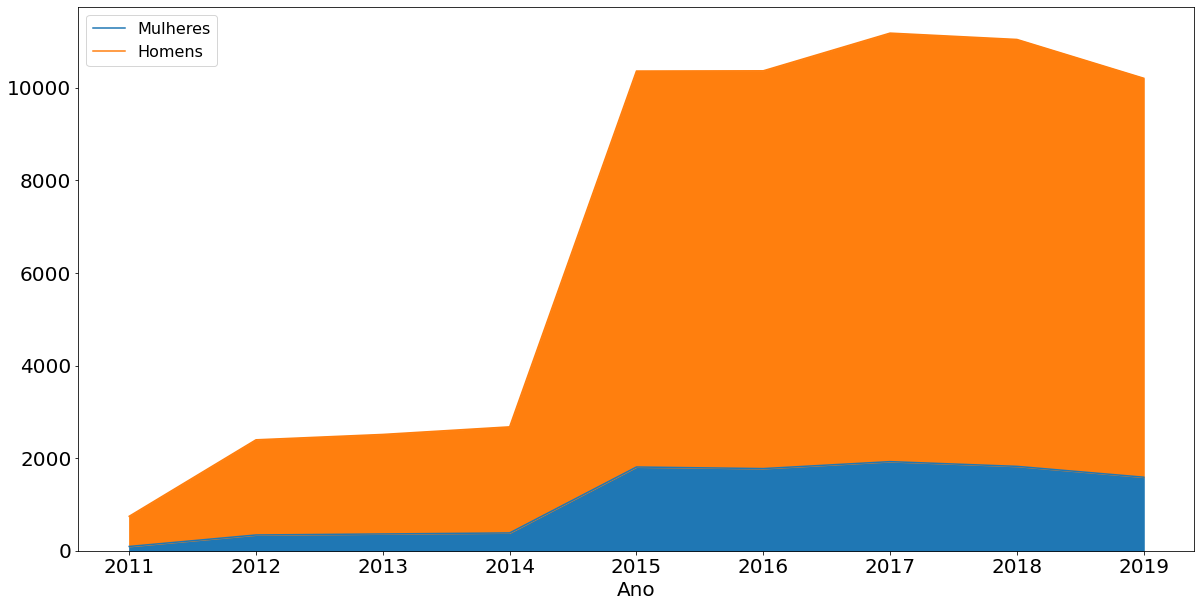
\includegraphics[width=1\textwidth]{Figuras/homensMulheresCincoProjetos.png}
\caption{Estudantes afetados por ano e gênero dos 5 projetos}
\label{fig:homensMulheresCincoProjetos}
\end{figure}

A Figura \ref{fig:homensMulheresCincoProjetos} considera o início do conjunto de projetos selecionados para contabilizar o número dos estudantes, por isso a alta no ano de 2015, onde dois projetos, WoMakersCode e Cunhantã Digital e Meninas Digitais Regional Mato Grosso, iniciaram.

\subsection{Participação em Atividade Extracurricular}\label{sub:extracurricular}

A Figura \ref{fig:extraCurricular} apresenta a participação dos estudantes em atividades extracurriculares. Apesar da nítida desigualdade, proporcionalmente de todos os homens 13,08\% fazem alguma atividade extracurricular, já as mulheres  13,43\% fazem alguma atividade. 

\begin{figure}[H]
\centering
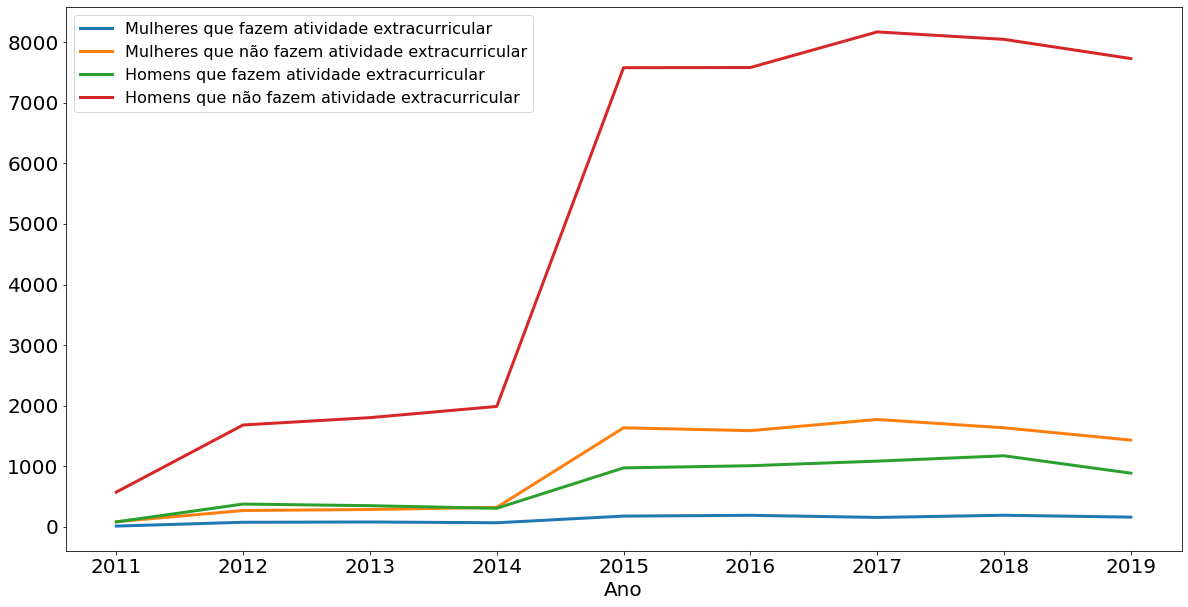
\includegraphics[width=1\textwidth]{Figuras/extraCurricular.png}
\caption{Participação em atividade extracurricular por gênero}
\label{fig:extraCurricular}
\end{figure}

A alta no ano de 2015, mais uma vez se dá pelo início dos projetos WoMakersCode e Cunhantã Digital. A Figura \ref{fig:extraCurricular} apresenta números absolutos de estudantes que participam ou não de atividade extracurricular no decorrer dos anos e como o número de homens é neste caso sempre superior ao número de mulheres, os homens também participam mais das atividades extracurriculares. 

% \subsection{Corpo Docente}\label{sub:docentes}

% Utilizando a mesma base do INEP e as IES de todas as análises anteriores, conforme o gráfico da Figura \ref{fig:professorGenero} a desigualdade de gênero também se apresenta no corpo docente.

% \begin{figure}[H]
% \centering
% 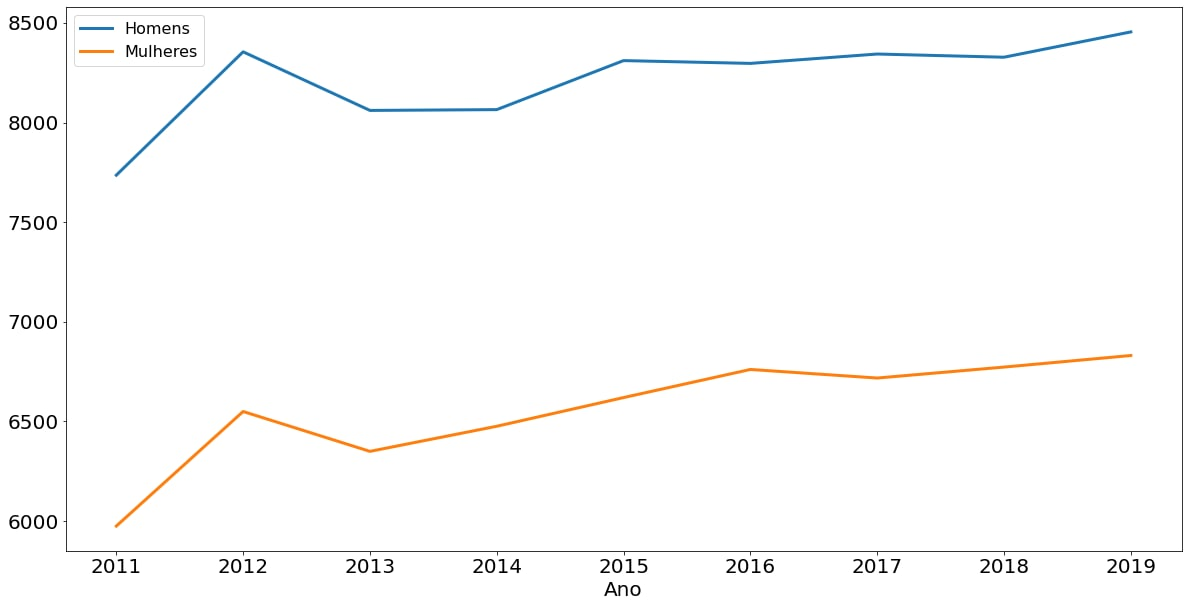
\includegraphics[width=1\textwidth]{Figuras/professores_sexo.jpeg}
% \caption{Participação em atividade extracurricular por gênero}
% \label{fig:professorGenero}
% \end{figure}

% Com a Figura \ref{fig:professorGenero} é de se estranhar o número alto de professores. Praticamente se igualando ao número dos alunos, porém as análises de corpo docente tornam-se dificultosas e limitadas por não existir a relação entre professor e curso, logo, as variáveis presentes na base do INEP sobre o corpo docente relacionam-se com a IES e não um curso específico.

% As variáveis presentes na base SUP\_DOCENTE do INEP são apenas variáveis da IES como código único de identificação da IES, tipo da categoria administrativa da IES e tipo da organização acadêmica da IES e variáveis do docente como escolaridade, gênero, regime de trabalho, data de nascimento e etc., não mencionando nada sobre curso. 


% %todas as análises sobre os projetos


\section{Entrevistas}\label{sec:Questionario}
%Questionário com foca na evasão.
%analises realizadas
Após todas as análises apresentadas na Seção \ref{sec:Avaliacoes} onde entende-se o panorama da presença de mulheres nos cursos de Computação e Tecnologias da Informação e Comunicação este trabalho também investigará por meio de entrevistas semi-estruturadas com pessoas dos projetos parceiros do Programa Meninas Digitais como estes projetos tem influenciado a presença e permanência de mulheres nos cursos de suas instituições.

O roteiro das entrevistas está sendo desenvolvido e terá perguntas para entender como o projeto interage com estudante, curso, instituição e corpo docente.

Este trabalho será submetido ao Comitê de Ética em breve. Todas as pessoas participantes deverão aceitar um Termo de Consentimento Livre e Esclarecido, apresentado no Apêndice \ref{ap:Termo}.

\section{Discussão do Capítulo}\label{sec:discussaoCapituloAnalises}
Neste capítulo foram apresentadas as análises sobre os dados do INEP do conjunto de projetos selecionados. As observações foram relacionadas aos estudantes, ano, gênero, idade, forma de ingresso e se eles participam ou não de atividades extracurriculares.

As análises apresentadas no capítulo podem ser continuadas em diversos outros gráficos e tabelas. Com isso pretende-se seguir e realizar novas análises, trazendo outras perspectivas e após as entrevistas, busca-se analisar a presença das mulheres nos cursos de TIC e a possível relação com as ações dos projetos parceiros do programa Meninas Digitais.